% File 'ugasample.tex' -- Michael A. Covington, Isidor Ruderfer (Revised 2007 April 11)
% This is an example of how to format a thesis or dissertation
% using LaTeX 2e with 'uga.sty' VERSION 3.2 OR LATER.



\documentclass[12pt]{report}

% If there are any other \usepackage commands, put them here


\usepackage{amsmath}
\usepackage{csquotes}
\usepackage{amssymb}
\usepackage{multirow}
\usepackage{booktabs}
\usepackage[style=authoryear,
backend=biber,
isbn=false,
maxcitenames=2,
mincitenames=1,
maxbibnames=99
]{biblatex}
\addbibresource{references.bib}
\usepackage{graphicx}
\graphicspath{ {./figs/} }

\DefineBibliographyStrings{english}{
  in = {}
}

\DeclareFieldFormat[article,inbook,incollection,inproceedings]{pages}{#1}
\DeclareFieldFormat{postnote}{#1}
\DefineBibliographyStrings{english}{
  techreport = {}
}

% DO NOT put any more \usepackage commands after \usepackage{uga}
\usepackage{uga}

% The following was recommended in the past so you can have hyperlinks in the eventual PDF output.
% It will produce profuse error messages when you have any unusual symbols or italics
% in a section title, or when you use pseudochapters.  Just ignore them.
% To activate it, remove the initial %.  In case of problems, put the % back in.
%\usepackage[ps2pdf, bookmarks=true, breaklinks=true]{hyperref}
% Note: As of 2008, this is NOT RECOMMENDED.  If you use it, check its effects carefully.

\title{Stochastic Valuation of Planted Loblolly Pine Stands Using Monte Carlo Simulation}

\author{Charles E. Merritt IV}

\previousdegrees{B.A., The University of Georgia, 2024}

\thisdegree{Master of Science}  % or Doctor of Philosophy, etc.

\thesistype{Thesis}     % or Dissertation

\thesismonth{July}       % put the graduation month here, not today's month...
\thesisyear{2026}

\professor{Pete Bettinger}

\fulltitle{Stochastic Valuation of Planted Loblolly Pine Stands Using Monte Carlo Simulation}

\indexwords{Forest Value, Forest Growth \& Yield Modeling, Simulation, Digital Forestry, Theses~(academic)}

\dean{Ron Walcott}

\memberi{Frederick Maier}
\memberii{Stephen Kinane}
\memberiii{Bruno Kanieski da Silva}

% Use \memberiii, \memberiv, \memberv for up to 3 more members if needed.

\usepackage[hidelinks]{hyperref} % or colorlinks=true,... see below
\hypersetup{
  bookmarksopen=true,
  bookmarksnumbered=true,
  pdfauthor={Charles E. Merritt IV},
  pdftitle={Stochastic Valuation of Planted Loblolly Pine Stands Using Monte Carlo Simulation}
}
\setcounter{tocdepth}{1} 

\makeatletter
\def\ps@myheadings{%
  \let\@mkboth\@gobbletwo
  \let\@oddhead\@empty
  \let\@evenhead\@empty
  \def\@oddfoot{\hfil\thepage\hfil}%
  \let\@evenfoot\@oddfoot
}
\def\ps@plain{%
  \let\@oddhead\@empty
  \let\@evenhead\@empty
  \def\@oddfoot{\hfil\thepage\hfil}%
  \let\@evenfoot\@oddfoot
}
\let\ps@headings\ps@plain
\let\ps@myheadings\ps@plain
\makeatother

\newcommand{\manualnumberedsection}[1]{%
  \refstepcounter{section}%
  \setcounter{subsection}{0}%
  \section*{\thesection\quad #1}%
  \phantomsection
  \addcontentsline{toc}{section}{\protect\numberline{\thesection}#1}%
}

\begin{document}
\pagenumbering{roman}
\pagestyle{plain}

\begin{abstract}
Stand-level forest planning is commonly conducted with deterministic growth and yield models that assume a single, idealized trajectory of stand development. However, forest stands evolve under substantial uncertainty arising from stochastic growth variation and disturbance events such as pests, wildfire, and wind damage. This thesis develops a modular stand simulation framework that augments an established deterministic loblolly pine (\textit{Pinus taeda}) growth model with stochastic process noise and probabilistic disturbance regimes, and uses Monte Carlo simulation to quantify how uncertainty alters economic valuation.

In this work, we evaluate a set of predefined, interpretable management prescriptions under both deterministic and stochastic dynamics. For each prescription and risk regime, repeated simulations generate a distribution of discounted cash flows and corresponding Net Present Value (NPV) and Land Expectation Value (LEV). Outcomes are summarized using measures of central tendency and dispersion as well as downside risk metrics, including Value at Risk (VaR) and Conditional Value at Risk (CVaR) to demonstrate tail-risk.

Results show that deterministic valuation can systematically mischaracterize stand value under uncertainty, particularly when low-probability, high-severity disturbances are possible. Across increasing disturbance frequencies and severities, the stochastic valuation distributions exhibit substantial tail risk and increased variability relative to deterministic baselines, and financially preferred rotation ages and prescriptions may shift accordingly. Collectively, these findings demonstrate the importance of distributional valuation in long-horizon timber management and provide a practical framework for comparing prescription robustness under stochastic disturbance regimes.
\end{abstract}


\maketitle    % Creates title page, copyright page if any, and approval page.


\chapter*{Dedication}
I dedicate this work to my mother, whose unwavering support and guidance have shaped me into the person I am today. Your belief in me has always been my greatest strength. To my siblings, Collier, Caiden, and Annalynn, your eyes inspire me daily to set a worthy example and continuously motivate me to become a better version of myself. Thank you all for keeping me grounded and focused on what truly matters.

\phantomsection
\pseudochapter{Acknowledgments}
This work was supported by the U.S. Department of Agriculture, National Institute of Food and Agriculture, Sustainable Agricultural Systems program, PERSEUS grant, {\#}2023-68012-38992. The findings and conclusions in this work have not been formally disseminated by the U. S. Department of Agriculture and should not be construed to represent any agency determination or policy. The U.S. Government is authorized to reproduce and distribute reprints for governmental purposes notwithstanding any copyright annotation therein.

\tableofcontents

\listoffigures   % Optional - Omit this line if you don't want a list of figures.
\listoftables    % Optional - Omit this line if you don't want a list of tables.

\newpage
\pagenumbering{arabic}  % Ordinary pages have Arabic numerals.

\chapter{Introduction}
\section{Background and Context}
Forest management decisions often span long time horizons, necessitating methods that anticipate future conditions and trade-offs. Yet most current stand-level planning models are deterministic, assuming a single, idealized trajectory of forest development. These models typically use optimization techniques to identify regimes that maximize a static objective (or set of objectives), most often timber volume or forest structure goals, though stands may also be managed for carbon sequestration, wildlife diversity, or recreation. In doing so, they often overlook a critical reality: forest stands are not deterministic environments.

Rather, forest stands are subject to stochastic and dynamic processes. Growth trajectories are influenced not only by competition and ecological succession, but also by random disturbances such as wildfires, windthrow, ice storms, and pest outbreaks. These events are often abrupt, severe, and difficult to predict. Weather modeling may provide insight into the likelihood of such events, but their occurrence remains inherently uncertain. Their effects propagate over time, altering successional pathways and disrupting static management plans. Despite this, such disturbances are often omitted from standard planning methods, which focus on idealized scenarios rather than risk-resilient strategies. Furthermore, disturbance events beyond a threshold of severity substantially increase the likelihood of subsequent disturbances. For example, woody debris caused by wind damage increases forest fuel loads and subsequently the likelihood of wildfire while also increasing the susceptibility of trees to infestation from pests such as pine beetles due to their weakened state.

These random disturbance events are projected to become more frequent and severe due to global climate change \parencite{marvelChapter2Climate2023}. The U.S. Southeast is expected to experience increased rainfall causing an increase in flash floods and rising nighttime heat levels are expected to increase storm severity \parencite{marvelChapter2Climate2023}. Recent history bears this out. For example, \textcite{helene_damage_assessment} reported that Hurricane Helene caused \$1.28 billion in damage to Georgia's forests, and affected up to 8.9 million acres of forest land in Georgia. Other events, such as the 2007 Georgia Bay Fire and the 2011 Honey Prairie Fire, burned 560,000 acres and 300,000 acres respectively. These events illustrate the vulnerability of forest systems to random, high-impact events in the southern United States.

The magnitude of this uncertainty calls for a new modeling paradigm, one that explicitly represents stochastic risks and allows agents to adapt to variable conditions over time. Rather than optimizing for a single, fixed trajectory, we propose a simulation-based framework that captures a range of plausible forest futures. While no simulator can perfectly reproduce the complexity of forest growth and disturbance, our intent is not to create a definitive predictive model for growth \textit{and} stochastic disturbances in timber stands. Instead, the simulation environment serves as a modular framework for evaluating management strategies and their effects on stand value under uncertainty. Its design allows for replacement or extension of the growth or disturbance models with site-specific or more sophisticated alternatives. By augmenting a deterministic growth and yield simulator with stochastic noise and disturbance events, we construct a flexible modeling environment in which multiple stochastic risk scenarios can be explored and evaluated against deterministic baselines.

To structure the stochastic elements in this environment, we model stand development as a probabilistic state transition process. At each annual timestep, stand attributes evolve according to established growth and yield equations, with additional variability introduced through stochastic process noise and disturbance events. This formulation allows us to generate multiple plausible realizations of stand development under identical management prescriptions.

Uncertainty in forest stand development can be categorized into two fundamental types. Aleatoric uncertainty arises from inherent randomness in natural processes, including annual growth variability, weather fluctuations, micro-site heterogeneity and the stochastic occurrence of disturbance events such as fire, wind, or pest outbreaks. This form of uncertainty is irreducible and must be propagated through simulation. Epistemic uncertainty, by contrast, stems from incomplete knowledge: imprecision in growth model parameters, limited calibration data, or structural assumptions about disturbance severity distributions. While epistemic uncertainty can in principle be reduced through additional data or improved models, it remains a practical constraint in operational forest planning. Our framework addresses both types: process noise and disturbance modules capture aleatoric variability, while scenario-based analysis and sensitivity testing quantify the influence of epistemic factors on management outcomes.

Risk is evaluated using distributional financial metrics rather than single point estimates. For each prescription and disturbance regime, Monte Carlo simulation produces a distribution of discounted cash flows and corresponding Net Present Value (NPV). These distributions are summarized using measures of central tendency and dispersion, as well as downside risk metrics such as Value at Risk (VaR) and Conditional Value at Risk (CVaR). This approach allows comparison not only of expected returns but also of resilience to rare but severe disturbance events.

By reframing stand valuation as a distribution rather than a deterministic forecast, this framework provides a more transparent view of the economic consequences of uncertainty. In doing so, it bridges classical deterministic growth and yield modeling with modern risk analysis, while remaining grounded in established forestry finance metrics such as NPV.

This thesis addresses several gaps: 
\begin{itemize}
\item The ubiquitous tendency to sidestep uncertainty in deterministic optimization models which leave out many probabilistic events that are relevant to growth but complicated to model as described by \textcite{stevensOptimalHarvestRates1986}.
\item The limited use of distributional valuation metrics in stand-level planning, where deterministic point estimates often mask downside risk.
\item The missing link between tried and true empirical stand growth models \parencite{pmrcHarrisonYieldPredictionGrowth1996} and stochastic models that include both probabilistic disturbances and growth factors.
\end{itemize}
We propose a framework that embraces stochasticity from the outset by embedding probabilistic disturbance processes within an established growth and yield model and evaluating heuristic ``rule of thumb'' management prescriptions through Monte Carlo simulation. This approach enables direct comparison between deterministic and stochastic valuation outcomes under varying disturbance regimes.

This thesis investigates how probabilistic disturbance modeling can be integrated with established growth and yield models to evaluate forest stand value under uncertainty.

\section{Stochastic vs. Deterministic Planning}
In this work we address key questions about the limitations of deterministic modeling of pine stand development.

    \textbf{How does deterministic stand valuation differ from stochastic valuation under identical management prescriptions?} \\
    This question evaluates the extent to which conventional deterministic planning methods, such as fixed-rotation management, diverge from valuation results obtained when stochastic disturbances and growth variability are explicitly modeled. We hold management prescriptions constant and examine how introducing stochastic disturbance processes alters expected value, variability, and downside risk compared to the deterministic case, and how different management regimes alter these outcomes.

    \textbf{How large is the bias introduced by ignoring disturbance risk and process uncertainty?} \\
    Deterministic stand models implicitly assume a single, idealized development trajectory. In contrast, stochastic Monte Carlo simulation generates a distribution of possible futures. This question assesses the difference between deterministic point estimates of value and the mean, median, and tail outcomes of the corresponding stochastic distribution. Particular attention is given to downside risk, including the probability of substantial loss under elevated disturbance regimes.

\section{Simulation and Valuation Framework}
In this work we address two important questions related to acknowledging uncertainty in pine stand development.

    \textbf{How can a stochastic stand simulator be structured to evaluate management prescriptions under uncertainty?} \\
    We model stand dynamics as a stochastic state transition process governed by mechanistic growth equations and probabilistic disturbance events. Management actions are specified through interpretable, rule-based prescriptions such as fixed rotation ages, thinning thresholds, and salvage responses. Rather than solving for an optimal policy through reinforcement learning, we simulate stand trajectories under each prescription across many Monte Carlo realizations to estimate the distribution of financial outcomes.

    \textbf{Which valuation and risk measures are appropriate for comparing deterministic and stochastic outcomes?} \\
    For each simulated trajectory, we compute discounted cash flows to obtain NPV, and when appropriate, LEV. Across Monte Carlo realizations, we summarize results using measures of central tendency and dispersion, as well as downside risk metrics such as VaR and CVaR. These measures allow comparison not only of expected returns but also of resilience to catastrophic loss. These risk measures are formally defined in the Evaluation Metrics section of Chapter 3.

Together, these questions clarify how incorporating stochastic disturbance processes changes economic valuation and prescription robustness in stand-level forest management.

\section{Modeling Assumptions}
Every model has underlying assumptions, and it's worth discussing them early and directly. First and foremost, while the methods presented are general, this work was conducted with managed, even-aged, loblolly pine (\textit{Pinus taeda}) plantations 
in mind. This simplifies the effort expended on factors such as species composition and competition. As such, our tree growth dynamics are modeled using region-specific equations provided by the Plantation Management Research Cooperative (PMRC). 
For the complete formulation of the deterministic growth model, see \textcite{pmrcHarrisonYieldPredictionGrowth1996}.

The stochastic kernel parameters that dictate the probability distributions for disturbances and growth variability are scenario-based, not empirically estimated. We explore uncertainty via structured parameter scenarios that span plausible ranges. All stochastic elements (e.g., disturbance probabilities, process noise intensity) are stationary within a scenario. The distribution parameters are chosen at the beginning and held fixed through the episode, which is equivalent to the rotation.

We use a fixed rotation age of 35 years, slightly longer than the standard economic rotation for southern pine plantations, to provide a consistent benchmark for comparing deterministic and stochastic outcomes. Discount rates, and management costs are also stationary and scenario-defined, they don’t evolve stochastically within a simulation. Stationarity is an important mathematical assumption for Markov processes, and the goal of this work is not to model the disturbance probabilities or economic factors themselves, but to understand the effect of these stochastic elements on stand value. For each of these values, we use the most recent estimates available from the literature.

Disturbances may have lagged effects (e.g., pest outbreaks causing gradual decline), which could be modeled with more complex recovery functions. In this work, disturbances do not alter future disturbance probabilities (e.g., one fire doesn’t reduce or increase the chance of another, except indirectly through changed stand state). When disturbances occur, a salvage fraction of 50\% of the timber volume is assumed available as revenue. This assumption is derived from the Georgia Forestry Commission's guidance on salvage logging operations \parencite{gfc_helene_recovery} and damage conditions following storms. Specifically, the 50\% fraction is based on the "moderate damage" level which describes conditions of a stand with a range of 20-50\% of damage. This value also maintains correspondence with the moderate severity kernel used in the disturbance module of the simulation framework.

Stumpage and action prices are also stationary and defined by the latest market research conducted by \textcite{costsMaggardNatzke}. We impose the following feasibility constraints: $\text{TPA} \geq 100$, $\text{BA} \geq 0$, $\text{HD}$ is non-decreasing, and $\text{Age} > 0$, where TPA is trees per acre, BA is basal area per acre (ft\textsuperscript{2}/acre), and HD is dominant tree height (ft).

Thinning, when applied as part of a fixed heuristic policy, is assumed to be ``from below'' to remove trees from the smallest size classes first. In the present work, we don’t model harvest scheduling constraints, road access, policy restrictions, or multi-stand interactions, as this is framed as a single stand modeling problem.

Finally, while the stand transition process is Markovian in structure, this assumption serves as a modeling abstraction rather than a literal claim about ecological memorylessness. The state vector is constructed to capture sufficient information for future growth and disturbance response within the scope of this study. It is very likely that the true ecological process is not Markovian, but this is a common assumption and is a useful abstraction for the purposes of this work.

\section{Thesis Statement}
This thesis demonstrates that deterministic growth-and-yield projections systematically overstate expected stand value when stochastic disturbances are present. Under identical management regimes and a 35-year rotation, Monte Carlo simulations ($n=1{,}000$) reveal that even modest disturbance frequencies---a 30-year mean return interval with 30\% mean severity---reduce mean LEV and NPV by 25\%. At higher but still realistic disturbance frequencies (10-year return interval), mean LEV declines by 63\% to \$545/acre. Process noise alone accounts for only a 5\% LEV reduction, indicating that discrete disturbance events---not growth variability---drive the valuation gap. These findings suggest that forest investment analyses relying solely on deterministic projections may substantially overestimate expected returns and understate downside risk.

\chapter{Related Works}

\section{Theoretical Framework}

This thesis develops a stochastic extension of a deterministic growth-and-yield model. The core modeling target is the distribution of terminal stand value under uncertainty:
\[
p(V_T \mid s_0, \pi, \theta)
\]
where $V_T$ is terminal timber value, $s_0$ is the initial stand state, $\pi$ is a fixed management policy, and $\theta$ parameterizes the stochastic transition kernel.

\subsection{Stochastic Transition Structure}

The stochastic transition factorizes as:
\[
P(s_{t+1} \mid s_t, a_t) = P(z_t) \cdot P(q_t \mid z_t) \cdot P(s_{t+1} \mid s_t, a_t, z_t, q_t)
\]
where $z_t \in \{0,1\}$ indicates disturbance occurrence and $q_t \in [0,1]$ is disturbance severity. $s_t$ is the stand state at time $t$ and $a_t$ is the management action at time $t$. A deterministic growth model provides the baseline transition $\mu_{t+1} = f(s_t, a_t)$, interpreted as the mean biological trend. The stochastic extension introduces two sources of uncertainty:

\begin{enumerate}
    \item \textbf{Process noise}: Multiplicative noise on growth increments, scaled by a global intensity parameter $\lambda_{proc}$. When this parameter is zero, the stochastic model reduces exactly to the deterministic baseline.
    \item \textbf{Disturbance events}: Discrete shocks with random occurrence and severity, applied as proportional reductions to state variables.
\end{enumerate}

This structure preserves the deterministic model as a limiting case while allowing systematic exploration of uncertainty regimes.

\subsection{Relationship to Markov Decision Processes}

While this framework can be viewed through the lens of Markov Decision Processes, several distinctions are important. First, the policy $\pi$ is a fixed heuristic rule, not an optimized or learned policy. Second, this is a forward stochastic simulator, not a Bayesian inference procedure or reinforcement learning algorithm. Third, epistemic uncertainty over stochastic kernel parameters is represented through structured scenarios rather than posterior distributions, as empirical calibration data were unavailable.

The Markov assumption serves as a modeling abstraction: the state vector is constructed to capture sufficient information for future growth and disturbance response within the scope of this study, though the true ecological process may exhibit longer memory.

\subsection{Simulation Target}

For fixed initial conditions, policy, and scenario parameters, the object of interest is the distribution of terminal value estimated via Monte Carlo simulation. This allows comparison of expected values, downside risk measures, and the probability of falling below deterministic benchmarks across uncertainty regimes. Specific distributional forms, parameter values, and experimental design are detailed in Chapter 3 (Methods).

\section{Current State of Knowledge}
\subsection{Net Present Value and Land Expectation Value}
The standard economic approach to optimizing the set of management decisions for an even-aged stand of pine trees (equivalently the ``management regime'' or the ``policy'' in an RL context) is to first determine the value of a single rotation for a stand and a given rotation age based on NPV.

The NPV of harvesting a forest stand at rotation age $T$ can be expressed as:

\[
NPV(T) = \sum_{t=0}^{T} \frac{R_t - C_t}{(1 + r)^t}
\]

where:
\begin{itemize}
    \item $R_t$ is the revenue received at time $t$ (e.g., from thinning or final harvest),
    \item $C_t$ is the cost incurred at time $t$ (e.g., planting, management, or treatment costs),
    \item $r$ is the discount rate,
    \item $T$ is the final rotation age.
\end{itemize}

Then, we expand on the definition of NPV to account for an infinite series of identical, even-aged rotations, starting from bare land. This is known as the Land Expectation Value (LEV). This formulation assumes that the same type of stand is regenerated and 
harvested infinitely many times on the same land. It can be expressed as:

\[
LEV(T) = NPV(T) \cdot \frac{(1 + r)^T}{(1 + r)^T - 1}
\]

where:
\begin{itemize}
    \item $NPV(T)$ is the net present value of one rotation of length $T$,
    \item $r$ is the discount rate,
    \item $T$ is the rotation age.
\end{itemize}

The optimal rotation age $T^*$ is defined as:

\[
T^* = \arg\max_{T} \, LEV(T).
\]


Once $T^*$ has been defined for a stand, it is constant for the foreseeable future as long as business proceeds ``as usual''. Finding $T^*$ is then a matter of some importance. It defines our ``infinite and identical rotations'' for the LEV. 
The standard method for establishing the optimal economic rotation age $T^*$ is to use the LEV to compare multiple rotation ages until the process converges on the rotation age that returns the highest value. There are other methods for determining the optimal rotation age, 
for instance one could use the biological method. In that case, when the mean annual increment is maximized, it is time to cut the stand. The mean annual increment (MAI) is calculated as:

\[
MAI(T) = \frac{V(T)}{T},
\]

where $V(T)$ is the total volume at age $T$. Both methods yield viable choices for the optimal rotation age, and there are many other viable methods. 
(For a more detailed examination of methods relating to the assignment of $T^*$ see \cite{BettingerAndLi2009}).

This method for calculating the value of a stand holds us to the assumption of ``infinite and identical rotations at the optimal rotation age'' in order to calculate the LEV. This assumption is extremely limiting, and in fact implicitly abstracts away uncertainty that might cause variance between two rotations. Nevertheless it remains an effective, easy, and robust way to calculate the economic value of a stand.

\subsection{Stochastic Forest Disturbance Modeling}
Accurate representation of forest disturbances is critical to keep our simulation as close as possible to the real dynamics of forest growth. To this end, we draw on the following references.
\begin{itemize}
\item ``A hierarchical simulation-through-optimization approach to forest disturbance modeling'' \parencite{campbellHierarchicalSimulationthroughoptimizationApproach2007}.
    This work offers insights into a Markov approach for forest-level modeling. They very simply alter the standard harvest scheduling approach by treating disturbances as if they were another type of harvesting activity with no revenue or cost. In this way, disturbed stands are implicitly seen as having no value. This method is general enough to allow them to ``model any stand-replacing disturbance...'' regardless of age. In calculating the likelihood of these disturbances for their spatial model, firstly they retrieved historical data for their study area that had similar rates of disturbances and harvest. Then, they discretize the likelihood of disturbance into decade-long bins, the same time-step used in their Markov model. \textcite{campbellHierarchicalSimulationthroughoptimizationApproach2007} offer a comprehensive methodology for defining a spatial Markov chain for forest-level modeling, especially with regards to an implementation of the disturbance events that is not overly complicated.
    
\item ``Optimal Harvest Rates Considering the Risk of Forest Fire'' \parencite{stevensOptimalHarvestRates1986}.
    This thesis deals with a single risk type and offers some guidance on the ways in which people have tried to solve these problems historically. Specifically, it compares a traditional ``even-flow'' model with a dynamic programming model to compare how fire-rate impacts harvest volumes.
    
\item ``Dealing with Non-linearity and Uncertainty in Forest Management'' \parencite{messierDealingNonlinearityUncertainty2016}.
This article argues for a shift in forest management from traditional ``command and control'' approaches toward viewing forests as complex adaptive systems that prioritize resilience and adaptability. The authors propose incorporating non-linearity and uncertainty into practices by moving management targets from strict stand-level outcomes to a broader ``envelope'' of acceptable conditions.

\item ``Stochastic or deterministic single-tree models: is there any difference in growth predictions?'' \parencite{fortinStochasticDeterministicSingletree2012}.
Critically, this paper shows that there are differences between stochastic and deterministic simulations due to interactions between ``nonlinear mechanisms underlying forest growth.'' 

\item ``Forest Growth and Yield Modeling'' \parencite{weiskittelForestGrowthYield2011}.
This textbook provides a comprehensive view of several major techniques for forest models, but also a sizable section on stand-level modeling as well. 
\end{itemize}

\subsection{Stand-Level Optimization Practices}
Stand-level optimization in forestry began in the 1970s using dynamic programming and simulation methods. Early work focused on determining the optimal rotation age for even-aged stands and designing thinning regimes to maximize timber value. The classical Faustmann rotation, which maximizes LEV under deterministic assumptions, remains the standard reference point for even-aged management. Extensions to the Faustmann framework introduced thinning schedules, variable discount rates, and non-timber objectives, but the underlying assumption of a single, known growth trajectory persisted.

Later, optimizing stand density became an important consideration. \textcite{bettingerDensitydependentStandlevelOptimization2005} developed a density-dependent stand-level optimization approach that derives management prescriptions by coupling growth simulators with nonlinear programming. Their work demonstrated that accounting for density-dependent mortality and competition effects materially changes optimal thinning intensity and timing relative to density-independent formulations.

A common limitation of these deterministic optimization approaches is that they assume the growth trajectory is known with certainty. When disturbance risk or growth variability is present, the single optimal prescription identified by deterministic methods may perform poorly across the range of plausible outcomes. This motivates the simulation-based approach adopted in the present study, where prescriptions are evaluated not by a single projected value but by the full distribution of outcomes under stochastic dynamics.

\subsection{Markov Decision Processes in Forest Modeling}
Markov Decision Processes (MDPs) provide a robust mathematical framework for modeling forest management under conditions of inherent ecological and economic risk. Unlike deterministic models that assume a known future, MDPs treat forest evolution as a series of stochastic transitions between discrete states. These states are typically defined by biophysical variables such as basal area, tree size, and species composition. With this in mind, the following three references are pertinent to this work.
\begin{itemize}
\item ``Managing Forests for Carbon and Timber: A Markov Decision Model of Uneven-aged Forest Management With Risk'' \parencite{johnstonManagingForestsCarbon2017}.
Focused on the Pacific Northwest, this study integrates carbon offset prices directly into an MDP objective function. It finds that moderate carbon prices enhance species and size diversity, but high prices may inadvertently promote monocultures as the forest is managed primarily for carbon.

\item ``A Graph-based Markov Decision Process approach for managing forests under risk of wind damage'' \parencite{forsellGraphbasedMarkovDecision2011}.
This article introduces Graph-based MDPs to address the spatial complexities of wind damage risk in Swedish forests. By accounting for how neighboring stands provide topographical shelter, the model optimizes management policies to increase the expected NPV of stands.

\item ``Adaptive economic and ecological forest management under risk'' \parencite{buongiornoAdaptiveEconomicEcological2015}.
This article presents an adaptive management framework for mixed stands in the southern U.S., it highlights that ignoring stochastic shocks leads to inaccurate ecological predictions. Using the theory of MDPs, the authors develop a framework for managing forests under uncertainty according to economic and ecological objectives.

\end{itemize}

\chapter{Methods}

\section{Research Design}

This study evaluates how deterministic and stochastic dynamics influence the economic valuation of a single forest stand under a fixed, rule-based management prescription. Rather than learning an optimal management policy under a continuous action space (through a process such as reinforcement learning), we specify a single heuristic basal-area-triggered thinning rule and compare financial outcomes under deterministic and stochastic growth scenarios.

The simulation framework models stand dynamics through annual state transitions over a 35-year rotation. The stand state $s_t = (a_t, h_t, n_t, b_t, S, r, \phi)$ consists of four dynamic variables---age ($a_t$), dominant height ($h_t$), trees per acre ($n_t$), and basal area ($b_t$)---and three constants: site index at base age 25 (S), physiographic region (r), and percent hardwood ($\phi$). Derived quantities such as volume and product yields are computed on-demand from these atomics. The stand is assumed to be even-aged and single-species (loblolly pine, \textit{Pinus taeda}), consistent with plantation conditions across the non-coastal areas of the southern United States.

Management is limited to a single heuristic thinning policy: thinning from below is triggered at age 15 when basal area exceeds 150 ft$^2$/ac, targeting a residual basal area of 100 ft$^2$/ac. Stumpage prices are fixed at \$9.51/ton (pulpwood), \$23.51/ton (chip-n-saw), and \$27.82/ton (sawtimber). Costs are also fixed: logging at \$150/acre, replanting at \$150.80/acre, and thinning at \$87.34/acre. Prices are derived from the latest TimberMarket South report, while costs are derived from the \textcite{costsMaggardNatzke} market report and online dashboard. A 5\% annual real discount rate is applied for NPV and LEV calculations.

The stochastic extension introduces two sources of uncertainty layered onto the deterministic PMRC model \parencite{pmrcHarrisonYieldPredictionGrowth1996}:
\begin{itemize}
    \item \textbf{Process noise}: Multiplicative lognormal noise on BA and HD increments, with mean correction ensuring $\mathbb{E}[\text{multiplier}] = 1$. TPA mortality uses a binomial model. A global scaling parameter $\lambda_{\text{proc}} \in \{0, 0.25, 0.5, 1.0\}$ controls noise intensity.
    \item \textbf{Disturbance events}: Annual Bernoulli occurrence with probability $p_{\text{dist}} \in \{0, 1/30, 1/20, 1/10\}$. Conditional severity follows $\text{Beta}(m_q \kappa, (1-m_q)\kappa)$ with $m_q = 0.30$ and $\kappa = 12$. Shocks are proportional reductions to TPA and BA; dominant height is unaffected.
\end{itemize}

When $\lambda_{\text{proc}} = 0$ and $p_{\text{dist}} = 0$, the stochastic model reduces exactly to the deterministic PMRC model projection baseline. This design ensures that differences in financial outcomes arise from uncertainty rather than model discrepancies.

The simulation environment consists of three primary components: a growth module, a disturbance module, and an economics module.

\manualnumberedsection{Management Prescriptions}

Management decisions are implemented through predefined, rule-based prescriptions rather than optimized control policies. Each prescription specifies treatment timing and intensity as a deterministic function of stand state variables. The prescriptions evaluated in this study include:

\textbf{Fixed Rotation (FR-T)} \\
A pine stand is harvested at a predetermined rotation age $T$. No intermediate treatments are applied unless explicitly specified. We evaluate a rotation age of 35 years to allow for an extended window into the dynamics of the stand.

\textbf{Basal Area Threshold Thinning (BAT)} 
A thinning from below is triggered when basal area exceeds a threshold $BA^*$. A fixed proportion $\tau$ of merchantable volume is removed at that time. Harvest occurs at a specified rotation age $T$.

Each prescription is applied identically across deterministic and stochastic simulations. This ensures that differences in financial outcomes arise from disturbance and growth variability rather than adaptive changes in management.

\manualnumberedsection{Growth Module}

We utilize the growth and yield model published in the report by \textcite{pmrcHarrisonYieldPredictionGrowth1996} to drive the core of the growth module. This work provides us with robust yield curves and growth equations that are the basis for the deterministic growth projections in our simulation framework.

For a time step $\Delta t = 1$ year, state variables are updated in the following order:
\begin{align}
    a_{t+1} &= a_t + \Delta t \\
    h_{t+1} &= f_h(a_t, h_t, a_{t+1}) && \text{(Chapman-Richards)} \\
    n_{t+1} &= f_n(n_t, S, a_t, a_{t+1}) && \text{(Survival equation)} \\
    b_{t+1} &= f_b(a_t, n_t, n_{t+1}, b_t, h_t, h_{t+1}, a_{t+1}, r) &&
\end{align}
This projection order respects the dependencies among state variables: age advances first, then height (which depends on age), then survival (which depends on site index and age), and finally basal area (which depends on all preceding variables).

The growth module is validated by running the deterministic simulator under representative initial conditions (SI$_{25}$=80, UCP region, TPA$_0$=850, age$_0$=5) and comparing the resulting trajectories to expected growth patterns for managed loblolly pine plantations in the Upper Coastal Plain. Over a 35-year rotation with basal-area-triggered thinning at age 15, the deterministic baseline produces a terminal harvest value of \$6{,}553/acre and an NPV of \$1{,}200/acre at a 5\% discount rate, yielding an LEV of \$1{,}465/acre. These values are consistent with published yield expectations for high-site-index loblolly pine under conventional management. Dominant height, basal area, and survival trajectories follow the expected sigmoid, asymptotic, and declining profiles respectively, and product class distributions at harvest age align with standard merchandising proportions. Separating growth from disturbance dynamics allows clear interpretation of baseline stand development prior to stochastic modification.

\manualnumberedsection{Disturbance Module}\label{sec:disturbance-module}

Disturbances are modeled as a generic category, rather than a specific disturbance such as fire, storm etc. Disturbances occur based on an annual Bernoulli trial and their severity is drawn from a Beta distribution, conditional on occurrence. The severity is used to determine the proportion of merchantable volume lost by applying a one-time shock to the atomic variables of the stand state and updating the state accordingly, and then checking for feasibility within the underlying growth model.

The occurrence of a disturbance in a given year is an independent Bernoulli trial with probability $p_{dist}$, where $p_{dist}$ is defined as the reciprocal of the mean return interval in years. This corresponds to a description of disturbances as ``occurring once every \textit{n} years'' where \textit{n} is the return interval.

\begin{table}[htbp]
  \centering
  \caption{Disturbance probability by return interval}
  \label{tab:disturbance_prob}
  \begin{tabular}{lc}
  \toprule
  Return Interval & $p_{\text{dist}}$ \\
  \midrule
  10 years & 0.10 \\
  20 years & 0.05 \\
  30 years & 0.033 \\
  None     & 0.00 \\
  \bottomrule
  \end{tabular}
\end{table}

Conditional on occurrence, disturbance severity $q_t$ is drawn from a Beta distribution with mean $m_q = 0.30$ and concentration $\kappa = 12$, parameterized as $\text{Beta}(m_q \kappa,\; (1-m_q)\kappa) = \text{Beta}(3.6,\; 8.4)$. A severity of 0.30 corresponds to a 30\% proportional reduction in both basal area and trees per acre. The concentration parameter $\kappa = 12$ produces a moderately peaked distribution: most disturbance events impose severity near the mean, but occasional draws above 0.50 or below 0.15 are possible. Dominant height is not reduced by disturbance shocks, reflecting the assumption that site productivity and top-height trees are more resistant to partial stand damage than aggregate density or stocking measures.

Figure~\ref{fig:severity-distribution} illustrates the shape of this severity distribution. The distribution is right-skewed ($\alpha < \beta$), with its mode at $q = 0.26$, median at $q = 0.29$, and mean at $q = 0.30$. The 75th percentile falls at $q = 0.38$, meaning that three-quarters of all disturbance events cause less than 38\% stand damage, while events exceeding 50\% severity occur in only about 5\% of draws. This parameterization is intended to represent a moderate, generic disturbance regime---consistent with the damage profiles commonly observed from ice storms, wind events, and minor insect outbreaks in managed loblolly pine stands in the southeastern United States. It does not attempt to capture the full severity spectrum of catastrophic events such as stand-replacing wildfire or major hurricane landfalls, which would require a heavier-tailed or bimodal severity model. Because the severity parameters are treated as scenario-based assumptions rather than empirically calibrated values, the concentration $\kappa$ could itself be varied in future sensitivity analyses to explore how the spread of the severity distribution affects financial outcomes.

\begin{figure}[htbp]
  \centering
  \includegraphics[width=\linewidth]{figs/severity_distribution.png}
  \caption{Probability density of the disturbance severity distribution, $\text{Beta}(3.6, 8.4)$. Dashed lines mark the mode, mean, median (p50), 75th percentile (p75), and 95th percentile (p95). The green shaded region indicates severities between the median and 75th percentile; the orange region indicates severities above the 75th percentile, which trigger the salvage action in the salvage sensitivity analysis.}
  \label{fig:severity-distribution}
\end{figure}

\manualnumberedsection{Economics and Cashflow Modeling}

The economics module converts simulated harvest and treatment decisions into annual cashflows. Revenues are calculated from harvested product classes using fixed stumpage prices. Treatment costs are assigned according to regional estimates \parencite{costsMaggardNatzke}.

Merchantable volume is partitioned into three product classes based on minimum DBH and top diameter specifications derived from standard southern pine merchandising rules. Table~\ref{tab:product_classes} summarizes the thresholds used. Product volumes are computed using the PMRC merchantability equations, which predict the fraction of whole-stand yield recoverable for each product specification. Exclusive volumes are obtained by subtraction: chip-and-saw volume is the yield meeting chip-and-saw specifications minus sawtimber yield, and pulpwood is the yield meeting pulpwood specifications minus chip-and-saw and above yield.

\begin{table}[htbp]
  \centering
  \caption{Product class specifications}
  \label{tab:product_classes}
  \begin{tabular}{lccc}
  \toprule
  Product Class & Min DBH (in) & Top Diameter (in) & Stumpage Price (\$/ton) \\
  \midrule
  Pulpwood      & 4.5 & 2.0 & 9.51 \\
  Chip-and-saw  & 8.5 & 4.0 & 23.51 \\
  Sawtimber     & 11.5 & 8.0 & 27.82 \\
  \bottomrule
  \end{tabular}
\end{table}

For each year $t$, net cashflow is defined as

\[
CF_t = \text{Revenue}_t - \text{Cost}_t.
\]

If a disturbance occurs, a salvage fraction of 50\% of damaged merchantable volume is assumed recoverable as revenue.

Financial performance over a rotation of length $T$ is evaluated using NPV:

\[
NPV = \sum_{t=0}^{T} \frac{CF_t}{(1+r)^t},
\]

where $r$ is the discount rate. When appropriate, LEV is derived from the rotation-level NPV to enable comparison with classical deterministic forestry benchmarks.

\manualnumberedsection{Evaluation Metrics}

For each management prescription and disturbance regime, Monte Carlo simulation produces a distribution of NPV outcomes. Results are summarized using:

\begin{itemize}
    \item Mean and median NPV,
    \item Standard deviation,
    \item Value at Risk (VaR) at $\alpha = 0.95$,
    \item Conditional Value at Risk (CVaR) at $\alpha = 0.95$,
    \item Probability of downside risk relative to the deterministic baseline.
\end{itemize}

VaR summarizes a lower-tail quantile of the simulated NPV distribution. For a chosen confidence level $\alpha$, $\mathrm{VaR}_{\alpha}$ is the threshold such that only $(1-\alpha)$ of outcomes are worse. In this setting, a 5\% VaR for NPV can be interpreted as a benchmark for unusually poor financial outcomes: across repeated stochastic simulations, approximately five percent of rotations produce an NPV below that level. VaR is useful because it converts a wide distribution of possible outcomes into a single, interpretable measure of downside exposure.

CVaR goes further by measuring the average outcome within that worst tail. Whereas VaR identifies where the lower tail begins, CVaR describes how severe losses are once that threshold has been crossed. This distinction is important for forestry applications because disturbance-driven losses are often highly asymmetric: many trajectories may remain near the deterministic baseline, while a relatively small number of severe fire, wind, or pest events generate disproportionately large economic damage. CVaR is therefore especially informative when the concern is not only the probability of bad outcomes, but also their average magnitude.

Together, VaR and CVaR complement mean and median NPV by distinguishing prescriptions that are profitable on average from those that are financially robust under adverse realizations. Two management prescriptions may have similar expected value but very different lower-tail behavior. Reporting these tail-risk measures makes it possible to compare prescriptions on resilience as well as return, which is central in a problem where rare but severe disturbances can dominate long-run economic performance.

We also report the probability of downside risk, defined as $P(\mathrm{NPV} < \mathrm{NPV}_{\text{det}})$, the fraction of Monte Carlo trajectories whose NPV falls below the deterministic baseline. This measure provides a direct, intuitive summary of how often stochastic outcomes underperform relative to the idealized projection. A downside probability near 1.0 indicates that deterministic valuation lies in the upper tail of the stochastic distribution and is therefore a poor representation of typical realized outcomes.

Deterministic valuation is obtained by running the same prescription with disturbance processes disabled. The difference between deterministic NPV and the Monte Carlo mean provides an estimate of bias introduced by ignoring stochastic risk.

This design allows direct comparison between deterministic planning assumptions and stochastic valuation outcomes, highlighting how disturbance frequency and severity alter expected returns and downside exposure.


\chapter{Results}

\section{Scenario Analysis}

For analysis of the stochastic model, we compare deterministic and stochastic trajectories under a shared management rule. Unless otherwise noted, each stochastic scenario is based on $n=1000$ Monte Carlo trajectories over a 35-year planning horizon. Thinning is applied as a deterministic trigger at age 15 when basal area exceeds 150 ft$^2$/ac, targeting a residual basal area of 100 ft$^2$/ac.

Figure~\ref{fig:catastrophe-comparison} illustrates the effect of disturbance frequency on mean stand trajectories. Increasing disturbance frequency reduces volume and basal area relative to the no-catastrophe baseline, as expected under repeated disturbance events. Trees per acre also declines more steeply under frequent disturbance because mortality shocks compound natural self-thinning. Dominant height is not shown because the model treats height as non-decreasing (disturbances do not reduce surviving tree heights), so HD trajectories are nearly identical across regimes. Volume provides an integrated summary of the cumulative production consequences of repeated disturbances, complementing the structural responses shown by basal area and TPA.

Figure~\ref{fig:product-distribution} shows an overview of stand development and per-product distribution in the deterministic case for an example 1 acre, even-aged pine stand in the Upper Coastal Plain region following an extended 40 year rotation. Additionally, the figure demonstrates revenue distribution across product classes and the undiscounted harvest profitability given only the fixed costs derived from \textcite{costsMaggardNatzke} and the cashflow from harvesting the stand at the end of the rotation. 

Figure~\ref{fig:thin-response} illustrates how the model handles the thinning response using a competition index. Following a thinning event, the residual stand exhibits an accelerated growth period relative to its pre-thin trajectory; however, this release response is bounded such that the thinned stand does not overtake the unthinned trajectory in basal area or volume. Accurately capturing thinning responses in southern pine stands remains an active area of research, and the approach used here prioritizes computational tractability and consistency with the deterministic growth engine over mechanistic detail. 

\begin{figure}[htbp]
  \centering
  \includegraphics[width=\linewidth]{figs/catastrophe_comparison.png}
  \caption{Mean growth trajectories under different catastrophe return intervals ($n=1000$ trajectories per scenario, $\lambda_{\text{proc}}=1.0$). Stand: SI$_{25}$=80, UCP region, TPA$_0$=850.}
  \label{fig:catastrophe-comparison}
\end{figure}


\begin{figure}[htbp]
  \centering
  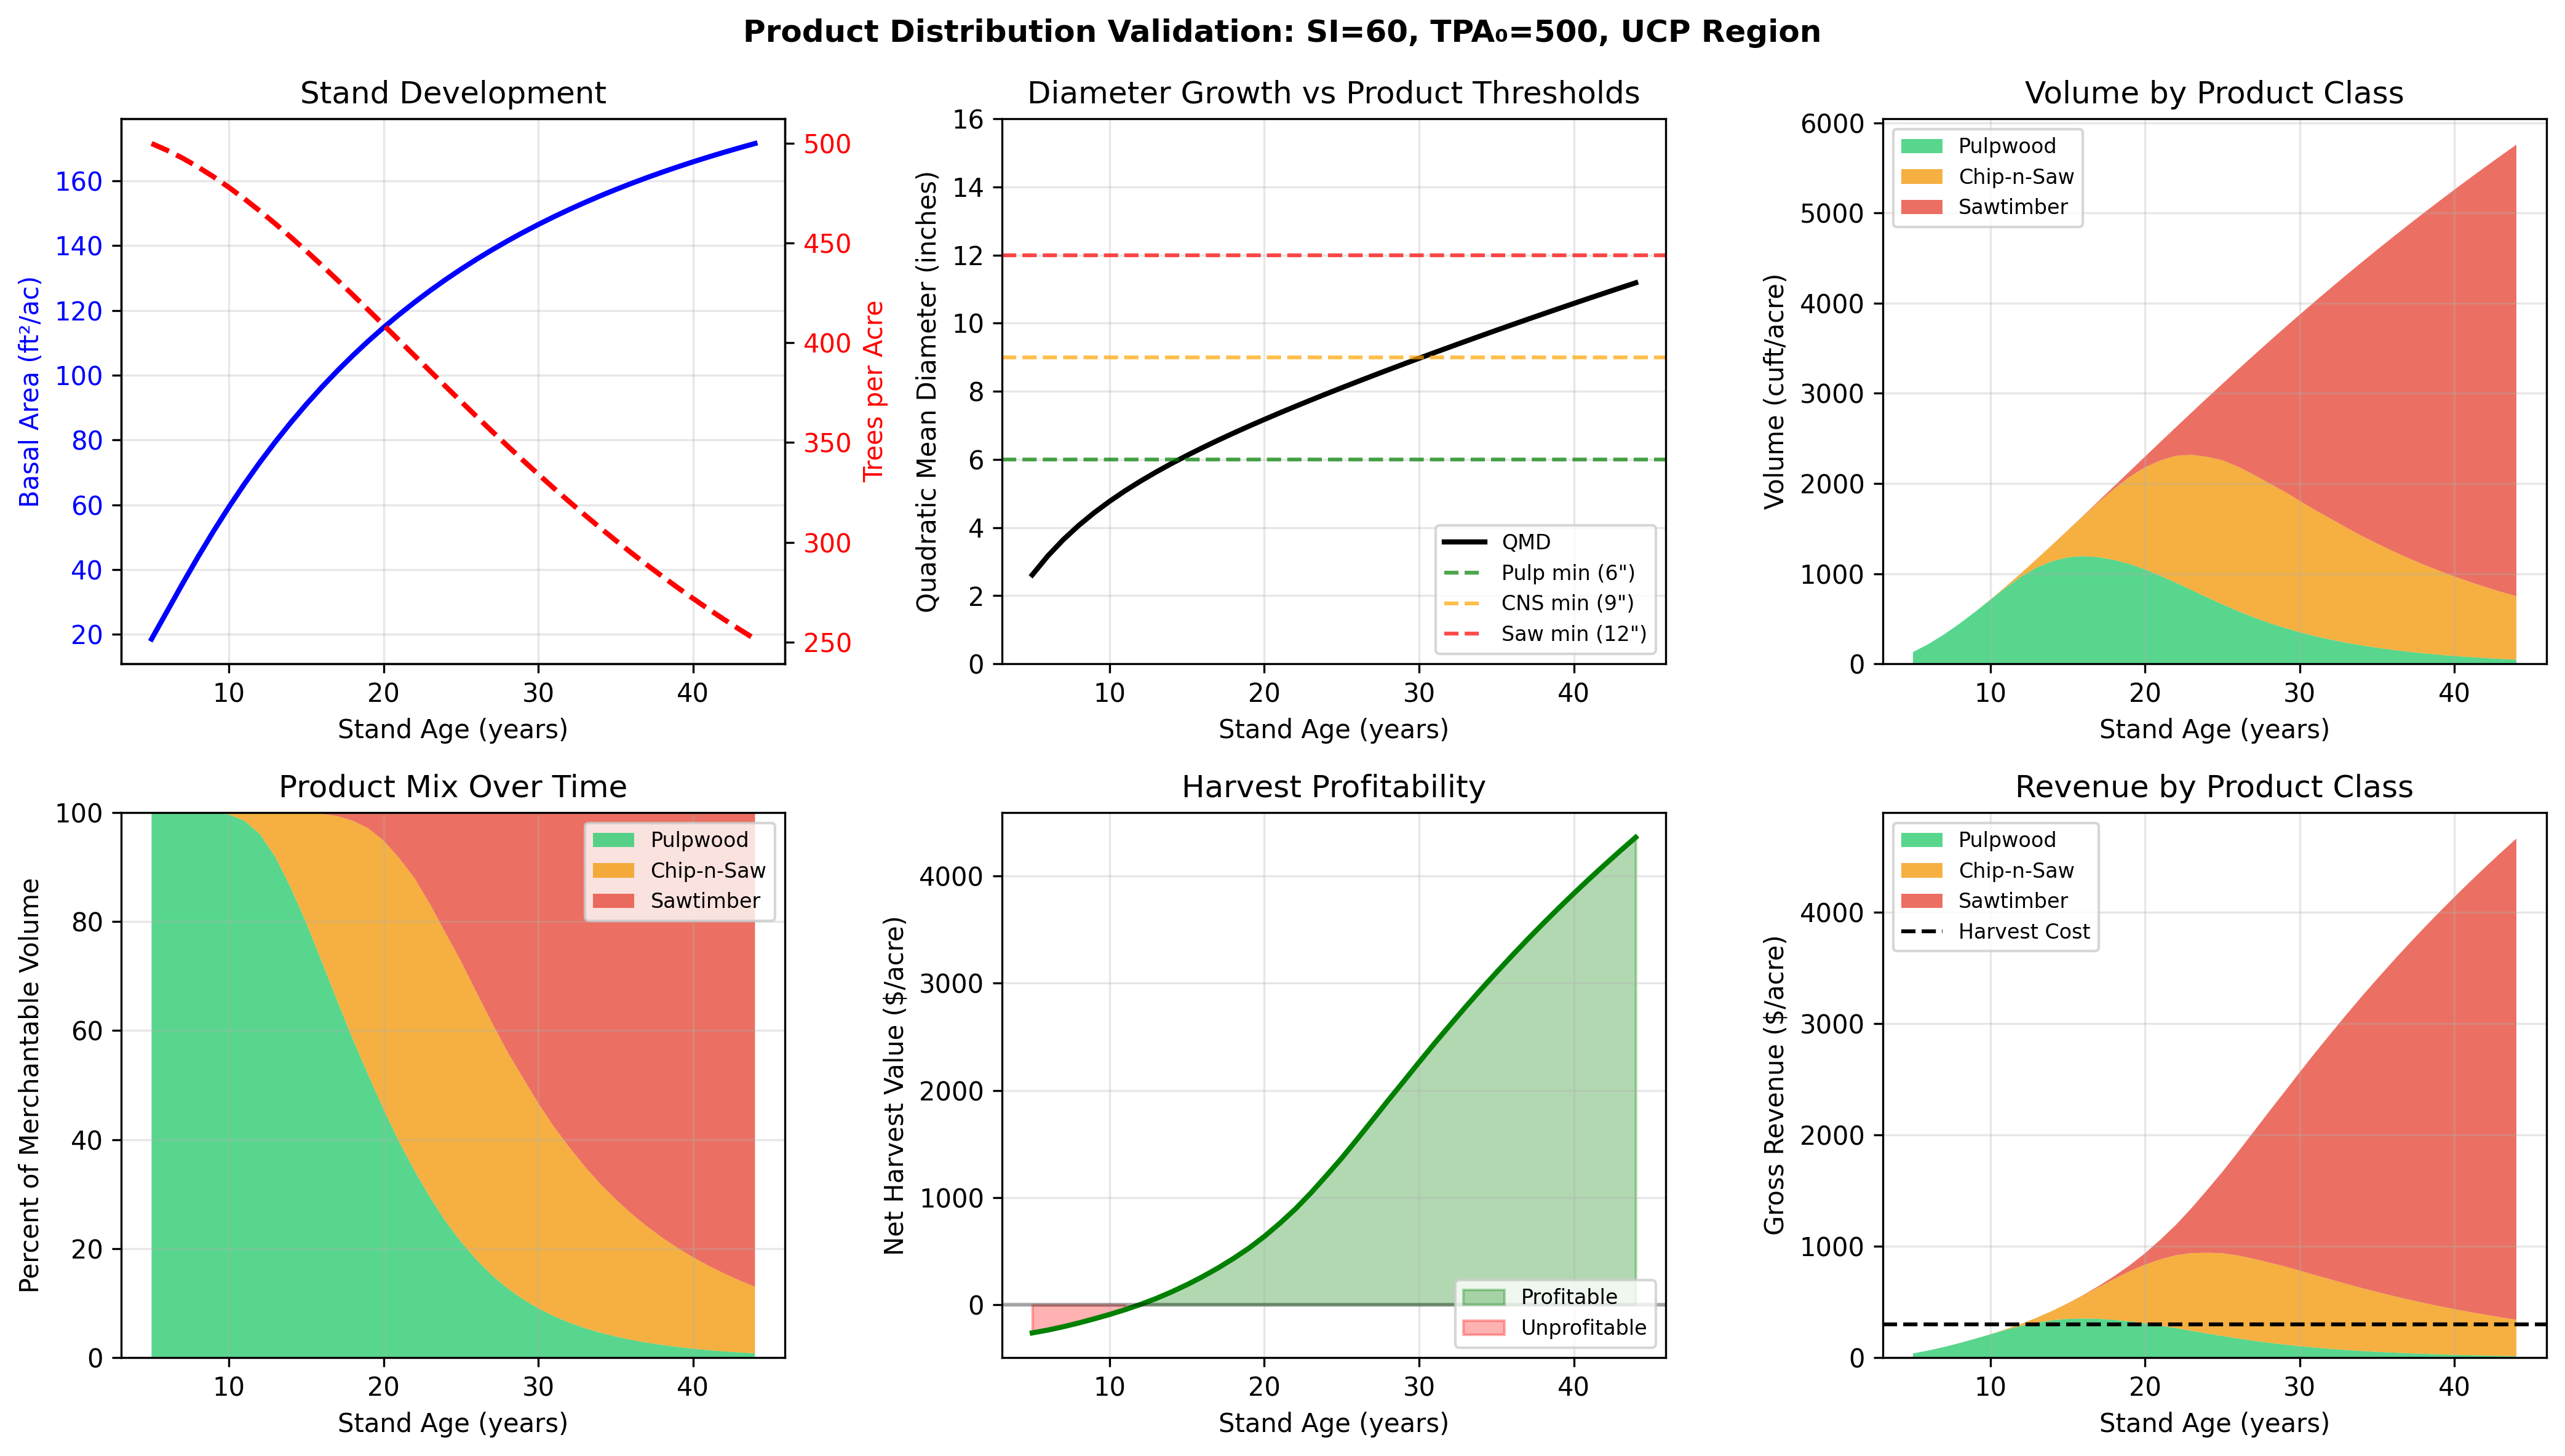
\includegraphics[width=\linewidth]{figs/product_distribution.png}
  \caption{Product distribution following extended rotation (40 years). Stand: SI$_{25}$=80, UCP region, TPA$_0$=850.}
  \label{fig:product-distribution}
\end{figure}

\begin{figure}[htbp]
  \centering
  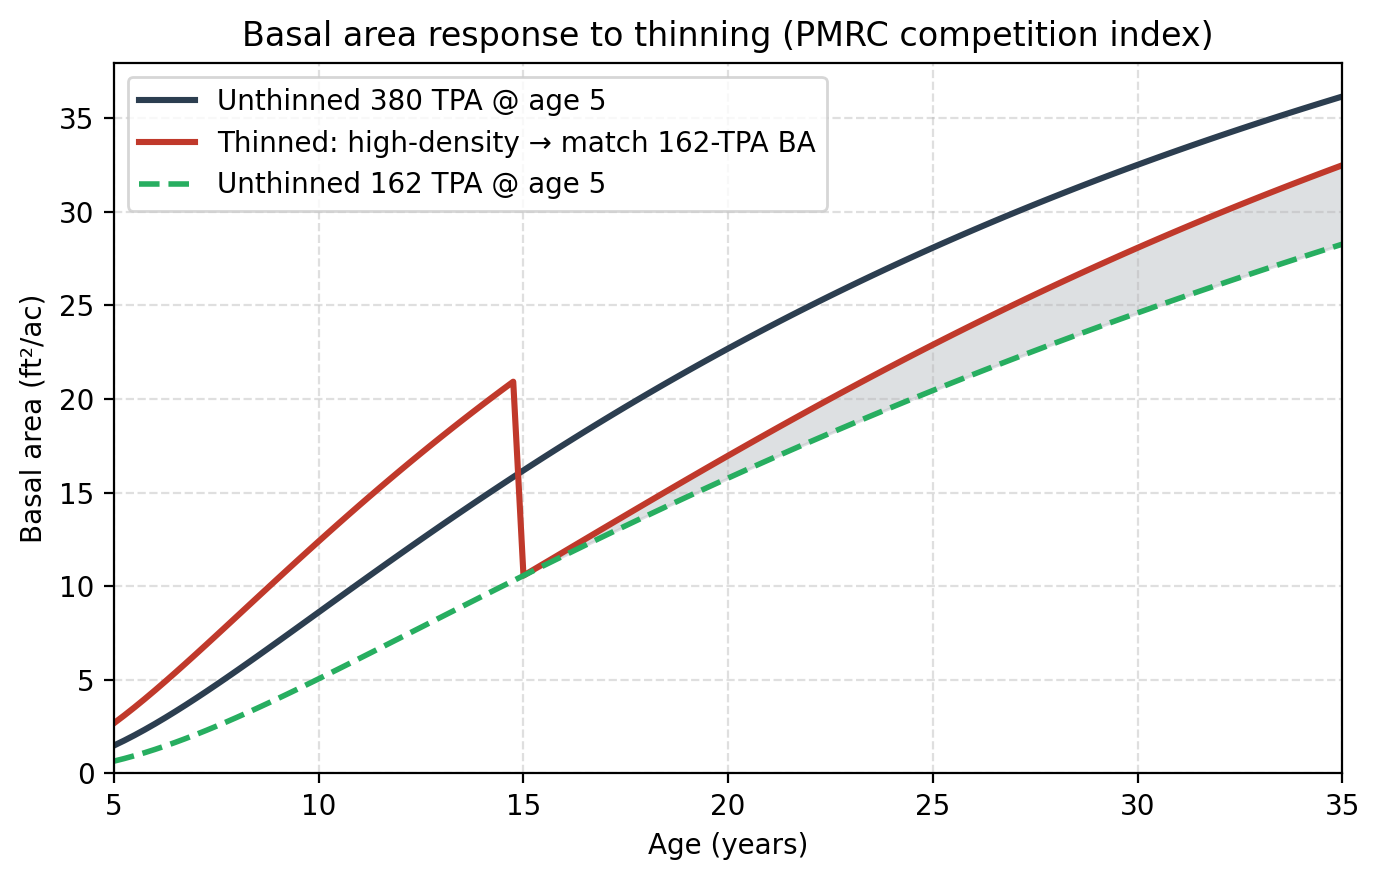
\includegraphics[width=\linewidth]{figs/thin_response.png}
  \caption{Deterministic thinning response relative to a 300-TPA unthinned reference baseline. Stand: SI$_{25}$=80, UCP region.}
  \label{fig:thin-response}
\end{figure}

\begin{table}[htbp]
  \centering
  \caption{Scenario naming convention}
  \label{tab:scenario_codes}
  \begin{tabular}{llcc}
  \toprule
  Code & Description & $\lambda_{\text{proc}}$ & $p_{\text{dist}}$ \\
  \midrule
  \texttt{deterministic} & Deterministic baseline & 0.00 & 0.00 \\
  \texttt{dist\_30} & Disturbance only, 30-yr return & 0.00 & 1/30 \\
  \texttt{dist\_20} & Disturbance only, 20-yr return & 0.00 & 1/20 \\
  \texttt{dist\_10} & Disturbance only, 10-yr return & 0.00 & 1/10 \\
  \texttt{noise\_025} & Process noise only ($\lambda=0.25$) & 0.25 & 0.00 \\
  \texttt{n025\_d30} & Low noise + 30-yr disturbance & 0.25 & 1/30 \\
  \texttt{n025\_d20} & Low noise + 20-yr disturbance & 0.25 & 1/20 \\
  \texttt{n025\_d10} & Low noise + 10-yr disturbance & 0.25 & 1/10 \\
  \texttt{noise\_050} & Process noise only ($\lambda=0.50$) & 0.50 & 0.00 \\
  \texttt{n050\_d30} & Moderate noise + 30-yr disturbance & 0.50 & 1/30 \\
  \texttt{n050\_d20} & Moderate noise + 20-yr disturbance & 0.50 & 1/20 \\
  \texttt{n050\_d10} & Moderate noise + 10-yr disturbance & 0.50 & 1/10 \\
  \texttt{noise\_100} & Process noise only ($\lambda=1.00$) & 1.00 & 0.00 \\
  \texttt{n100\_d30} & Full noise + 30-yr disturbance & 1.00 & 1/30 \\
  \texttt{n100\_d20} & Full noise + 20-yr disturbance & 1.00 & 1/20 \\
  \texttt{n100\_d10} & Full noise + 10-yr disturbance & 1.00 & 1/10 \\
  \bottomrule
  \end{tabular}
\end{table}

Figure \ref{fig:npv-boxplots} summarizes NPV distributions across the full factorial of process noise intensity ($\lambda_{\text{proc}}$) and disturbance probability ($p_{\text{dist}}$). As either source of uncertainty increases, median NPV declines and interquartile range widens. The deterministic baseline (dashed line) lies above nearly all stochastic medians, confirming that ignoring uncertainty systematically overstates expected returns. Figure \ref{fig:product-distribution} shows several validation metrics for the deterministic scenario in terms of stand development and product distributions. Figure \ref{fig:thin-response} shows the manner in which thinning response is handled in the model using a competition index. Figure \ref{fig:npv-heatmap} presents mean NPV as a heatmap over the same parameter grid. The gradient from upper-left (low noise, low disturbance) to lower-right (high noise, high disturbance) illustrates the compounding effect of both uncertainty sources on expected stand value.

\begin{figure}[htbp]
  \centering
  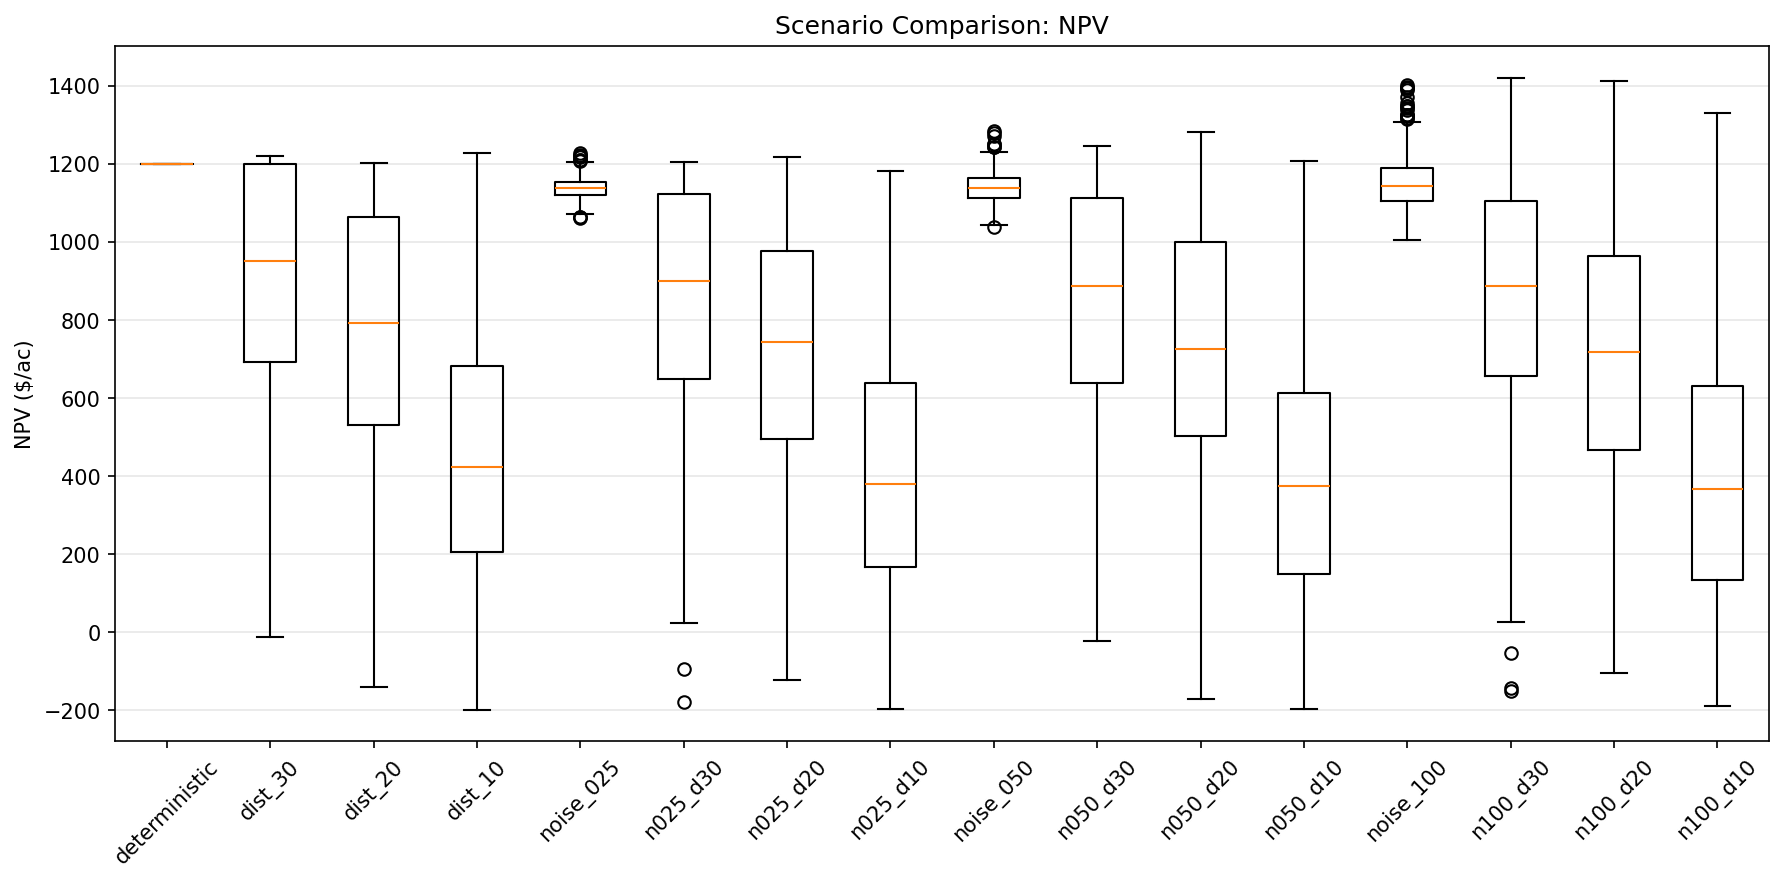
\includegraphics[width=\linewidth]{../data/experiment_results/figures/npv_boxplots.png}
  \caption{NPV distributions across scenarios defined by process noise intensity and disturbance probability ($n=1000$ trajectories per scenario). Stand: SI$_{25}$=80, UCP region, TPA$_0$=850. Dashed line indicates deterministic baseline.}
  \label{fig:npv-boxplots}
\end{figure}

\begin{figure}[htbp]
  \centering
  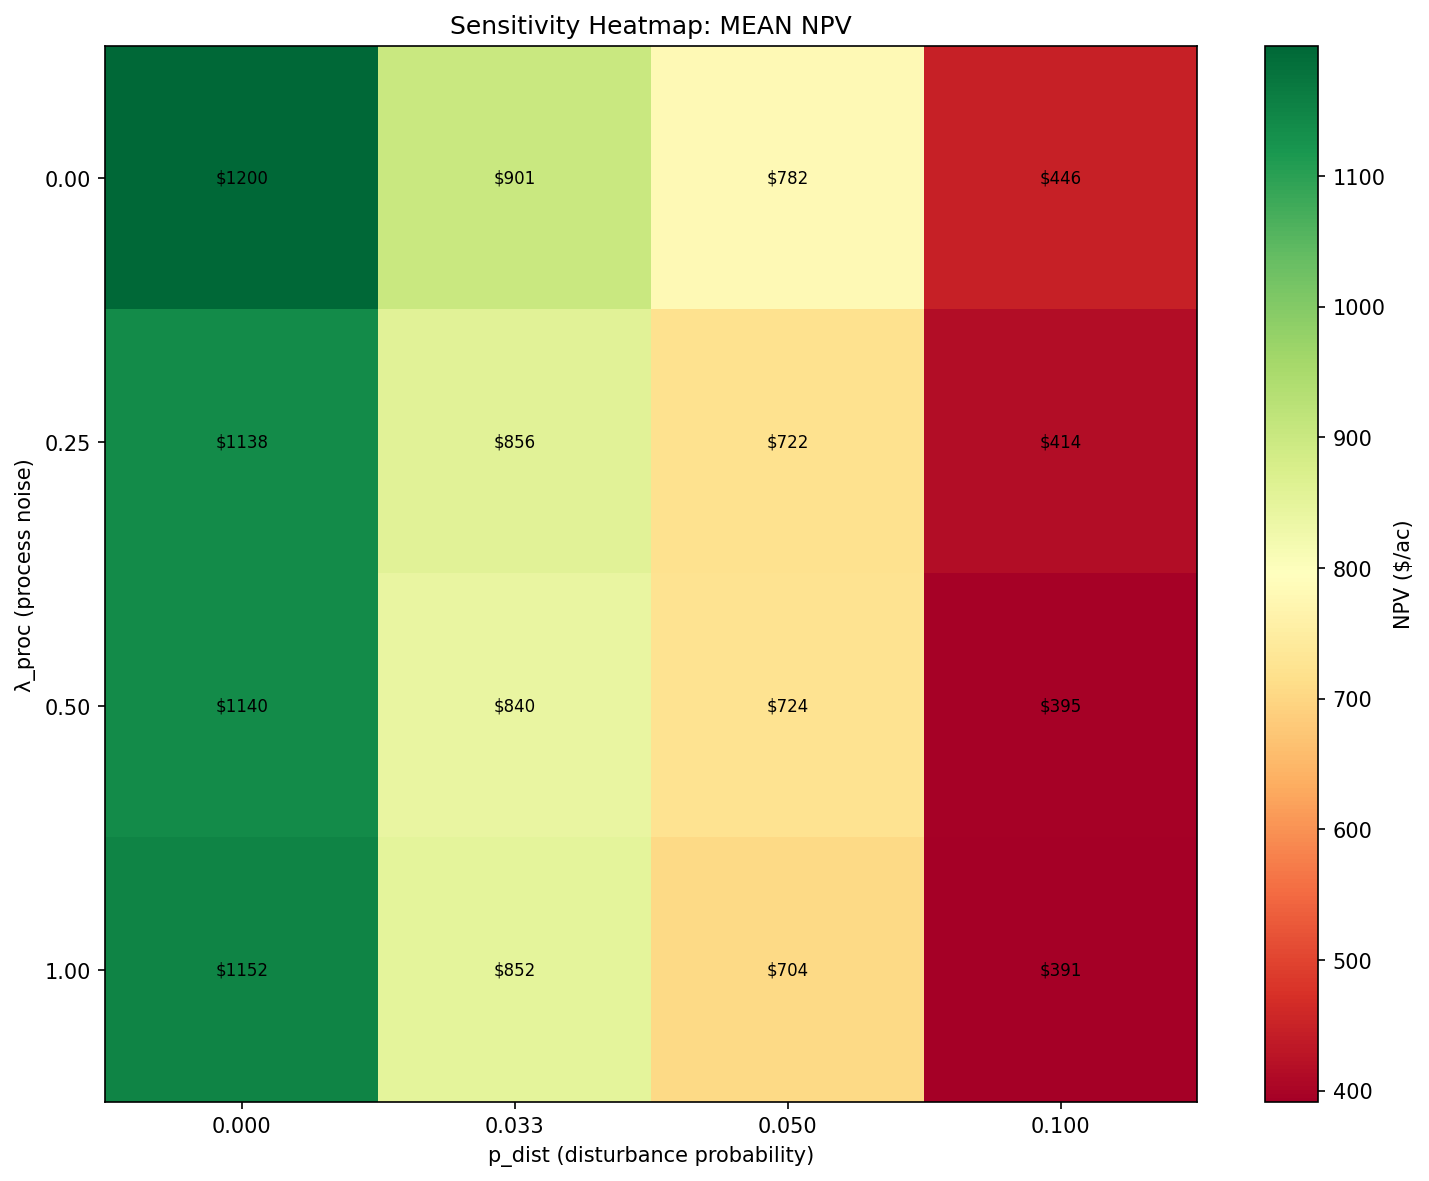
\includegraphics[width=0.8\linewidth]{../data/experiment_results/figures/npv_heatmap_mean.png}
  \caption{Mean NPV heatmap across process noise intensity ($\lambda_{\text{proc}}$) and disturbance probability ($p_{\text{dist}}$). Stand: SI$_{25}$=80, UCP region, TPA$_0$=850.}
  \label{fig:npv-heatmap}
\end{figure}

Terminal harvest value distributions (Figure \ref{fig:terminal-value-boxplots}) show a similar pattern. Under high disturbance frequency, the distribution becomes increasingly left-skewed as severe disturbance events truncate stand development before merchantable volume accumulates.

\begin{figure}[htbp]
  \centering
  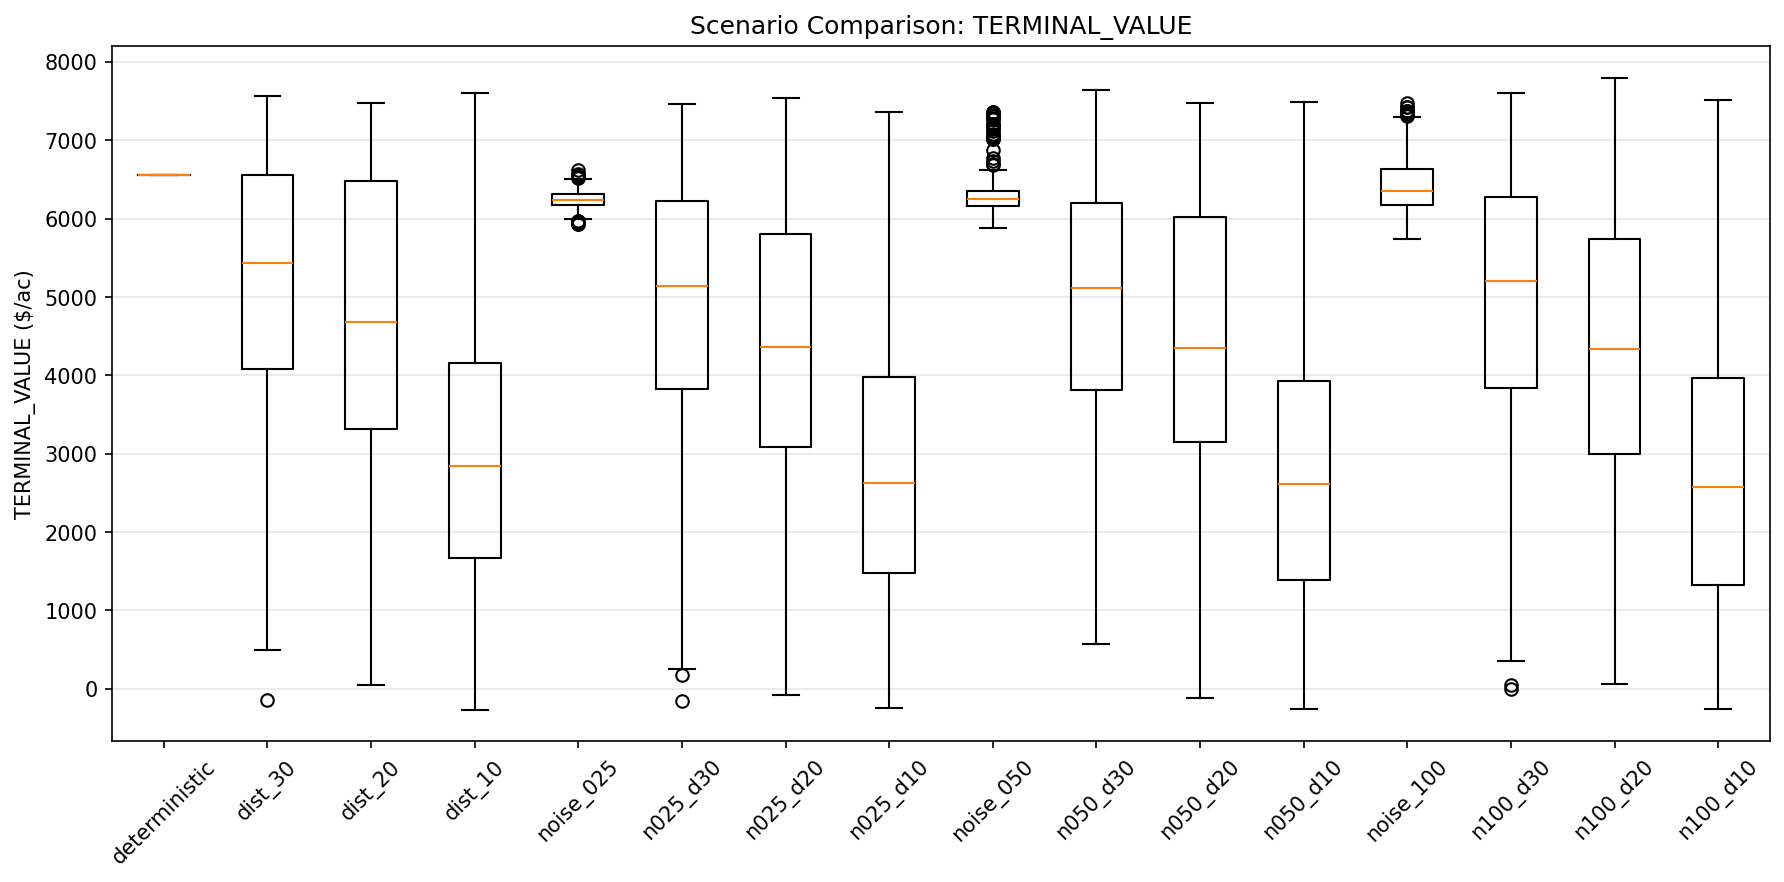
\includegraphics[width=\linewidth]{../data/experiment_results/figures/terminal_value_boxplots.png}
  \caption{Terminal harvest value distributions across scenarios ($n=1000$ trajectories per scenario). Stand: SI$_{25}$=80, UCP region, TPA$_0$=850.}
  \label{fig:terminal-value-boxplots}
\end{figure}

The shape of the terminal value distribution shifts with disturbance regime. Figure \ref{fig:hist-baseline} shows the distribution under moderate uncertainty ($\lambda_{\text{proc}}=0.50$, $p_{\text{dist}}=1/20$), while Figure \ref{fig:hist-high-dist} shows the distribution under elevated disturbance risk ($\lambda_{\text{proc}}=0.50$, $p_{\text{dist}}=1/10$). The latter exhibits a heavier lower tail, reflecting increased probability of substantial value loss.

\begin{figure}[htbp]
  \centering
  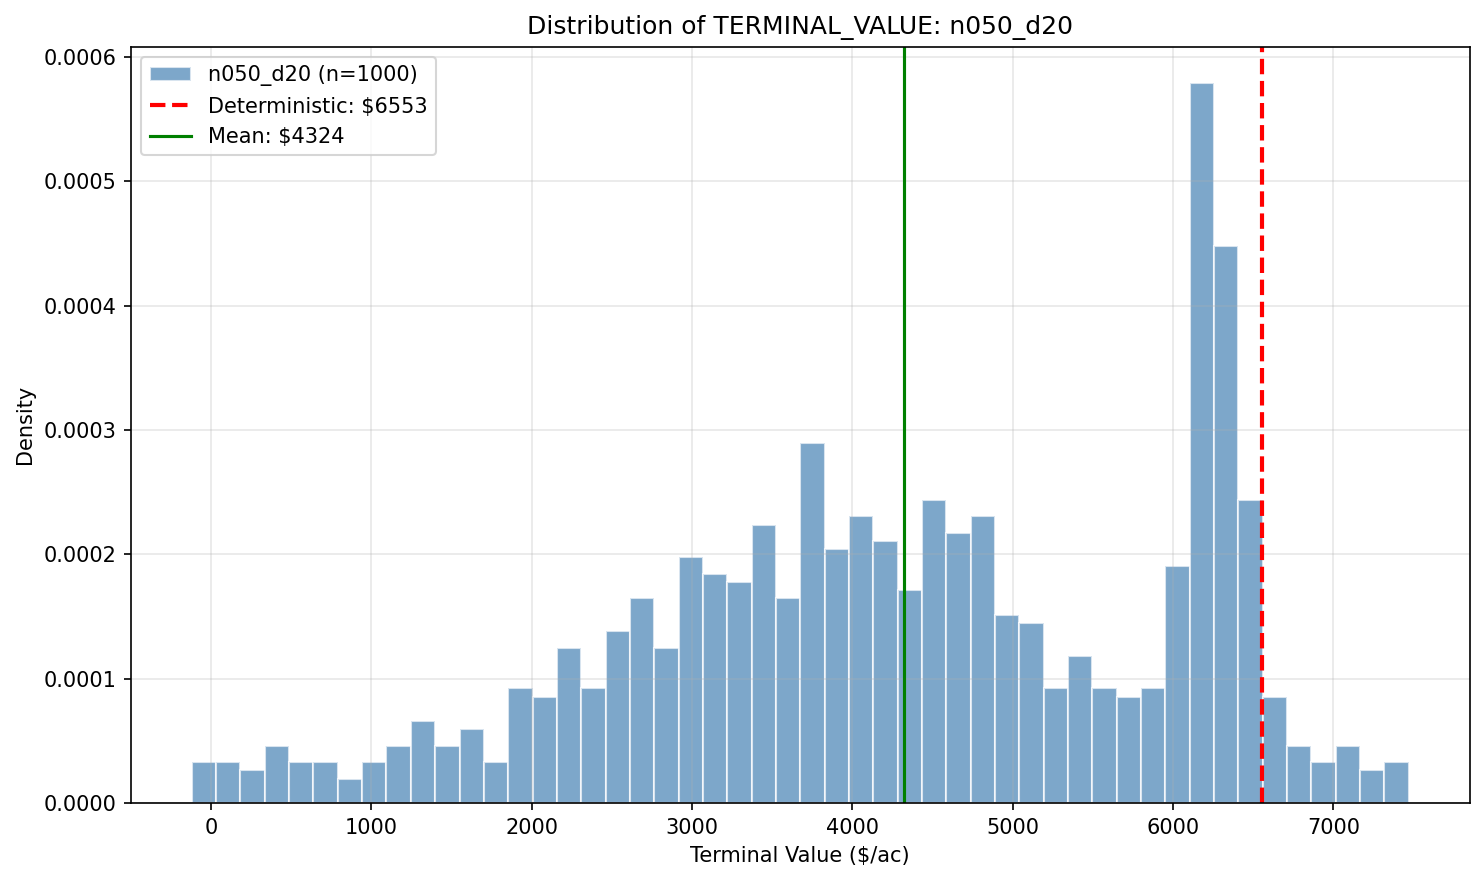
\includegraphics[width=0.8\linewidth]{../data/experiment_results/figures/histograms/n050_d20_terminal_value_histogram.png}
  \caption{Terminal value distribution under moderate uncertainty ($\lambda_{\text{proc}}=0.50$, $p_{\text{dist}}=1/20$, $n=1000$). Stand: SI$_{25}$=80, UCP region, TPA$_0$=850.}
  \label{fig:hist-baseline}
\end{figure}

\begin{figure}[htbp]
  \centering
  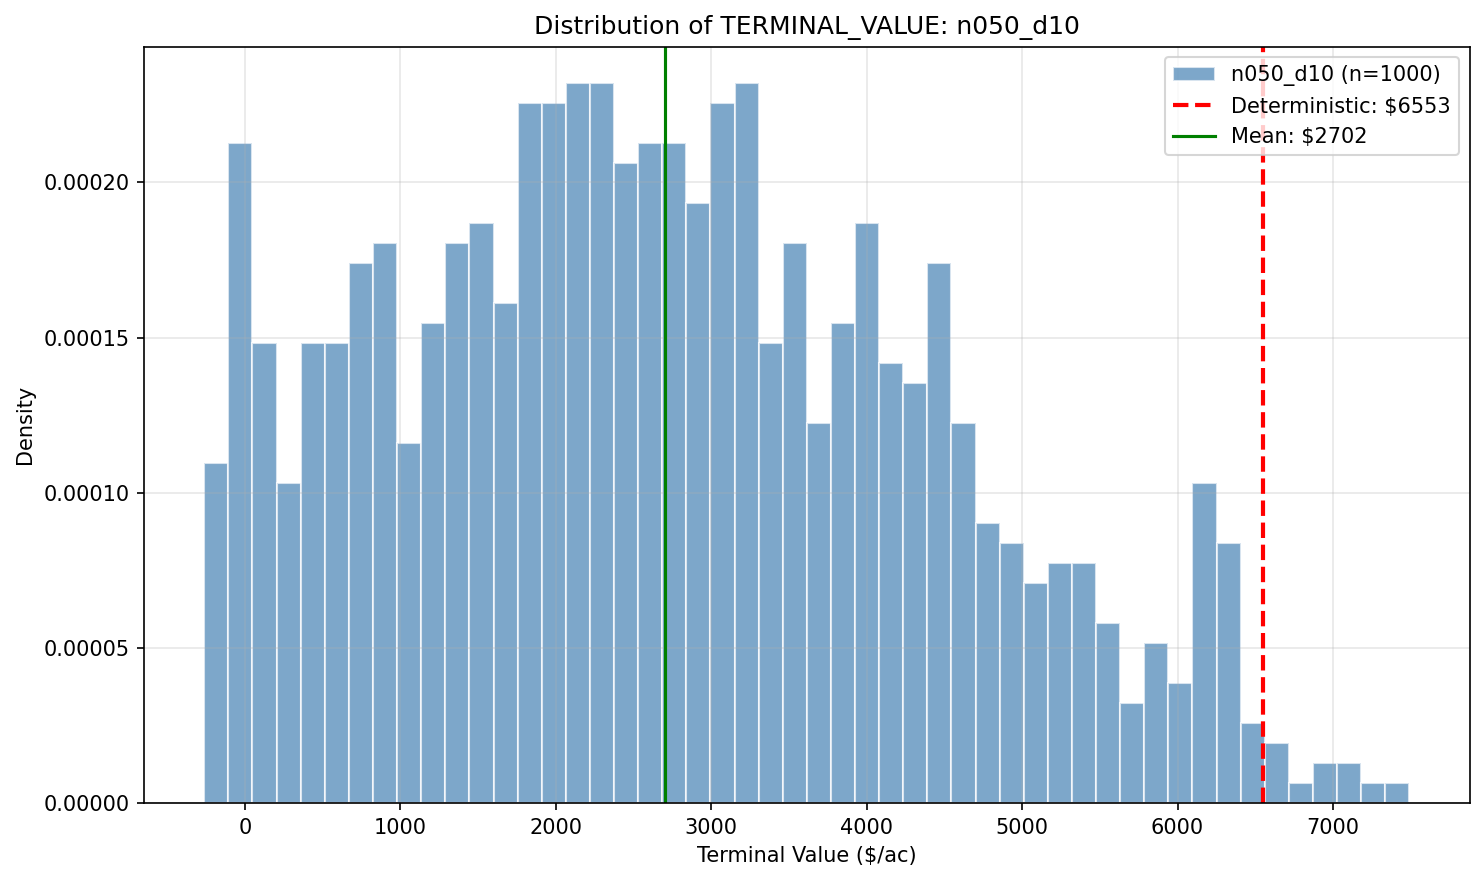
\includegraphics[width=0.8\linewidth]{../data/experiment_results/figures/histograms/n050_d10_terminal_value_histogram.png}
  \caption{Terminal value distribution under elevated disturbance risk ($\lambda_{\text{proc}}=0.50$, $p_{\text{dist}}=1/10$, $n=1000$). Stand: SI$_{25}$=80, UCP region, TPA$_0$=850.}
  \label{fig:hist-high-dist}
\end{figure}

The full set of terminal value histograms for all stochastic scenarios is provided in the appendix.

Table~\ref{tab:npv_summary} reports summary statistics for the NPV distribution across all scenarios. The deterministic baseline produces an NPV of \$1{,}200/acre. Under disturbance-only regimes, mean NPV declines from \$901/acre (30-year return interval) to \$446/acre (10-year return interval). Process noise alone introduces modest dispersion but has limited effect on the mean: even at full noise intensity ($\lambda_{\text{proc}}=1.0$), mean NPV remains within 4\% of the deterministic value. When both sources of uncertainty are active, mean NPV is dominated by disturbance frequency rather than noise intensity. The 5\% VaR and CVaR columns reveal substantial tail risk under elevated disturbance regimes. For example, under \texttt{n050\_d10}, the 5\% VaR is $-$\$121/acre and CVaR is $-$\$159/acre, indicating that the worst 5\% of trajectories produce negative returns. Downside probability exceeds 0.93 in every scenario that includes disturbance, confirming that the deterministic projection consistently overstates realized value.

\begin{table}[htbp]
  \centering
  \caption{NPV summary statistics by scenario (\$/acre, $n=1000$ trajectories). Stand: SI$_{25}$=80, UCP region, TPA$_0$=850.}
  \label{tab:npv_summary}
  \small
  \begin{tabular}{lrrrrrrr}
  \toprule
  Scenario & Mean & Median & Std Dev & 5\% VaR & CVaR$_{5\%}$ \\
  \midrule
  \texttt{deterministic} & 1{,}200 & 1{,}200 & 0 & 1{,}200 & 1{,}200 \\
  \texttt{dist\_30}      & 901  & 951  & 290 & 357  & 228 \\
  \texttt{dist\_20}      & 782  & 792  & 318 & 243  & 145 \\
  \texttt{dist\_10}      & 446  & 424  & 329 & $-$83  & $-$140 \\
  \texttt{noise\_025}    & 1{,}138 & 1{,}139 & 25  & 1{,}099 & 1{,}087 \\
  \texttt{n025\_d30}     & 856  & 899  & 278 & 338  & 208 \\
  \texttt{n025\_d20}     & 722  & 743  & 308 & 189  & 96 \\
  \texttt{n025\_d10}     & 414  & 380  & 333 & $-$90  & $-$150 \\
  \texttt{noise\_050}    & 1{,}140 & 1{,}139 & 38  & 1{,}076 & 1{,}067 \\
  \texttt{n050\_d30}     & 840  & 888  & 287 & 290  & 193 \\
  \texttt{n050\_d20}     & 724  & 726  & 320 & 142  & 19 \\
  \texttt{n050\_d10}     & 395  & 374  & 326 & $-$121 & $-$159 \\
  \texttt{noise\_100}    & 1{,}152 & 1{,}144 & 65  & 1{,}061 & 1{,}044 \\
  \texttt{n100\_d30}     & 852  & 887  & 292 & 317  & 184 \\
  \texttt{n100\_d20}     & 704  & 718  & 326 & 141  & 41 \\
  \texttt{n100\_d10}     & 391  & 367  & 336 & $-$120 & $-$155 \\
  \bottomrule
  \end{tabular}
\end{table}

Table~\ref{tab:lev_summary} presents corresponding LEV statistics. The deterministic LEV is \$1{,}465/acre. Under the 30-year disturbance return interval, mean LEV falls to \$1{,}100/acre---a 25\% reduction. At the 10-year return interval, mean LEV drops to approximately \$545/acre, a 63\% decline, with 97\% of trajectories falling below the deterministic benchmark. These LEV results confirm the NPV findings at the infinite-rotation scale and are consistent with the thesis statement.

\begin{table}[htbp]
  \centering
  \caption{LEV summary statistics by scenario (\$/acre, $n=1000$ trajectories). Stand: SI$_{25}$=80, UCP region, TPA$_0$=850.}
  \label{tab:lev_summary}
  \small
  \begin{tabular}{lrrrrrrr}
  \toprule
  Scenario & Mean & Median & Std Dev & 5\% VaR & CVaR$_{5\%}$ \\
  \midrule
  \texttt{deterministic} & 1{,}465 & 1{,}465 & 0 & 1{,}465 & 1{,}465 \\
  \texttt{dist\_30}      & 1{,}100 & 1{,}162 & 354 & 436  & 278 \\
  \texttt{dist\_20}      & 955  & 967  & 388 & 297  & 177 \\
  \texttt{dist\_10}      & 545  & 518  & 402 & $-$101 & $-$171 \\
  \texttt{noise\_025}    & 1{,}390 & 1{,}391 & 30  & 1{,}342 & 1{,}328 \\
  \texttt{n025\_d30}     & 1{,}046 & 1{,}098 & 340 & 413  & 255 \\
  \texttt{n025\_d20}     & 882  & 907  & 376 & 231  & 117 \\
  \texttt{n025\_d10}     & 505  & 464  & 406 & $-$110 & $-$183 \\
  \texttt{noise\_050}    & 1{,}392 & 1{,}392 & 47  & 1{,}314 & 1{,}303 \\
  \texttt{n050\_d30}     & 1{,}026 & 1{,}085 & 351 & 354  & 236  \\
  \texttt{n050\_d20}     & 885  & 887  & 391 & 173  & 23  \\
  \texttt{n050\_d10}     & 482  & 457  & 398 & $-$147 & $-$195 \\
  \texttt{noise\_100}    & 1{,}407 & 1{,}397 & 79  & 1{,}296 & 1{,}276 \\
  \texttt{n100\_d30}     & 1{,}041 & 1{,}083 & 357 & 387  & 225  \\
  \texttt{n100\_d20}     & 860  & 877  & 399 & 173  & 50 \\
  \texttt{n100\_d10}     & 478  & 449  & 410 & $-$146 & $-$190 \\
  \bottomrule
  \end{tabular}
\end{table}

\section{Salvage Sensitivity Analysis}

The preceding results demonstrate that disturbance risk substantially reduces expected stand value. A natural question is whether a reactive management action---salvage harvesting---can recover some of this lost value. In this analysis, salvage is modeled as a severity-triggered stand reset: when a disturbance event exceeds a specified severity threshold, the manager clearcuts the remaining post-disturbance volume at a reduced stumpage price, pays logging and replanting costs, and resets the stand to initial conditions (age$_0$=5, TPA$_0$=850, SI$_{25}$=80). Salvage is not a conventional harvest; it is an emergency response that recovers partial value from a damaged stand rather than allowing the degraded stand to continue growing.

To assess the robustness of salvage across different disturbance environments, we evaluate two severity distributions (Figure~\ref{fig:severity-comparison}). The moderate regime, $\text{Beta}(3.6, 8.4)$, has mean severity $m_q = 0.30$ and is right-skewed, with most events causing 15--38\% stand damage and only 5\% of events exceeding 53\% severity. The extreme regime, $\text{Beta}(3, 3)$, has mean severity $m_q = 0.50$ and is symmetric, with substantially fatter tails: 25\% of events exceed 64\% damage and 5\% exceed 81\%. The extreme regime represents a scenario in which disturbance events are reliably destructive, as might occur under compounding stressors such as drought-weakened stands exposed to beetle outbreaks followed by wind damage.

\begin{figure}[htbp]
  \centering
  \includegraphics[width=\linewidth]{figs/severity_distribution_comparison.png}
  \caption{Disturbance severity distributions used in the salvage sensitivity analysis. Left: moderate regime, $\text{Beta}(3.6, 8.4)$, with mean 0.30 and right skew. Right: extreme regime, $\text{Beta}(3, 3)$, with mean 0.50 and symmetric shape. Shaded regions indicate the p50--p75 range (green) and above-p75 range (orange). Summary statistics are inset.}
  \label{fig:severity-comparison}
\end{figure}

\subsection{Salvage Threshold Sensitivity}

Table~\ref{tab:salvage-threshold} reports mean NPV across four salvage threshold conditions---no salvage, and salvage triggered at the 25th, 50th, and 75th percentiles of the severity distribution---under both severity regimes and three disturbance frequencies. The salvage price fraction is held at 50\% of normal stumpage for all salvage conditions.

\begin{table}[htbp]
  \centering
  \caption{Mean NPV (\$/acre) by salvage severity threshold and disturbance regime ($n=1000$ trajectories, salvage price = 50\% of stumpage). Stand: SI$_{25}$=80, UCP region, TPA$_0$=850.}
  \label{tab:salvage-threshold}
  \small
  \begin{tabular}{llrrrr}
  \toprule
  Severity Regime & $p_{\text{dist}}$ & No Salvage & p25 & p50 & p75 \\
  \midrule
  \multirow{3}{*}{Moderate: Beta(3.6, 8.4)}
    & 1/30 & 689 & 663 & 694 & \textbf{704} \\
    & 1/20 & 567 & 548 & 588 & \textbf{593} \\
    & 1/10 & 262 & 253 & 314 & \textbf{326} \\
  \midrule
  \multirow{3}{*}{Extreme: Beta(3, 3)}
    & 1/30 & 510 & 566 & \textbf{577} & 556 \\
    & 1/20 & 351 & 430 & \textbf{435} & 411 \\
    & 1/10 &  30 & 103 & \textbf{123} & 103 \\
  \bottomrule
  \end{tabular}
\end{table}

Under the moderate severity regime, the p75 threshold consistently produces the highest mean NPV, with improvements of \$15--\$64/acre over no salvage that scale with disturbance frequency. Critically, the p25 threshold is \textit{value-destroying}: it reduces mean NPV below the no-salvage baseline in every disturbance regime. This occurs because the p25 threshold ($q \geq 0.205$) triggers salvage on mild disturbance events where only 20--25\% of the stand is damaged---damage the stand can grow through without intervention. In these cases, the replanting cost (\$150.80/acre) and the lost growth from resetting to age 5 outweigh the partial salvage revenue. The p50 threshold yields intermediate results, modestly improving NPV but underperforming p75 because it still triggers on below-average-severity events that do not justify a stand reset. These results indicate that under a moderate severity distribution, salvage is only economically justified for severe events in the upper tail.

The pattern reverses under the extreme severity regime. Here, the p50 threshold consistently outperforms p75, producing the highest mean NPV in all three disturbance regimes. The improvement is dramatic under frequent disturbance: at $p_{\text{dist}} = 1/10$, salvage at the median threshold raises mean NPV from \$30/acre to \$123/acre, compared to only \$103/acre at p75. This reversal occurs because the extreme distribution is symmetric around $m_q = 0.50$, so the median event causes 50\% stand damage. At this severity level, post-disturbance recovery is slow and costly relative to the option of resetting. Even the p25 threshold ($q \geq 0.359$) is value-positive under the extreme regime, because a 36\% damage event under $\text{Beta}(3, 3)$ is far more destructive in context than the same proportional loss under the moderate distribution, where the stand retains more structural integrity for regrowth.

\subsection{Salvage Price Fraction Sensitivity}

Table~\ref{tab:salvage-price} reports mean NPV across four salvage price conditions---no salvage, and salvage at 25\%, 50\%, and 75\% of normal stumpage price---with the severity threshold held at p75 for all salvage conditions.

\begin{table}[htbp]
  \centering
  \caption{Mean NPV (\$/acre) by salvage price fraction and disturbance regime ($n=1000$ trajectories, threshold = p75). Stand: SI$_{25}$=80, UCP region, TPA$_0$=850.}
  \label{tab:salvage-price}
  \small
  \begin{tabular}{llrrrr}
  \toprule
  Severity Regime & $p_{\text{dist}}$ & No Salvage & 25\% Price & 50\% Price & 75\% Price \\
  \midrule
  \multirow{3}{*}{Moderate: Beta(3.6, 8.4)}
    & 1/30 & 689 & 678 & 704 & \textbf{732} \\
    & 1/20 & 567 & 557 & 593 & \textbf{631} \\
    & 1/10 & 262 & 274 & 326 & \textbf{384} \\
  \midrule
  \multirow{3}{*}{Extreme: Beta(3, 3)}
    & 1/30 & 510 & 551 & 556 & \textbf{563} \\
    & 1/20 & 351 & 405 & 411 & \textbf{421} \\
    & 1/10 &  30 &  96 & 103 & \textbf{113} \\
  \bottomrule
  \end{tabular}
\end{table}

Under the moderate severity regime, the salvage price fraction has a substantial effect on NPV. At 25\% of stumpage, salvage is approximately break-even or slightly value-destroying: the salvage revenue barely covers the replanting cost after discounting, producing results close to or below the no-salvage baseline. At 75\% of stumpage, the benefit is pronounced---under $p_{\text{dist}} = 1/10$, mean NPV rises from \$262/acre (no salvage) to \$384/acre, an improvement of \$122/acre. This indicates that the economic viability of salvage under moderate severity depends critically on how much of the damaged timber's value can be recovered at market. The price fraction captures real-world variability in salvage timber markets: severely damaged timber may be sold at deep discounts due to quality degradation, limited buyer interest, and urgency of removal, while moderately damaged timber may retain most of its value.

Under the extreme severity regime, salvage is value-positive at all price fractions, including the lowest (25\%). This reflects the fact that under $\text{Beta}(3, 3)$, severe disturbance events leave the stand so damaged that even a low-revenue salvage harvest followed by replanting outperforms passive recovery from a 60--80\% loss. However, the marginal value of moving from 50\% to 75\% price is smaller under the extreme regime (\$7--\$10/acre) than under the moderate regime (\$28--\$58/acre), because the primary value of salvage in the extreme case comes from the stand reset rather than the timber revenue itself.

\chapter{Discussion}
The central result of this study is that disturbance risk changes both expected value and the shape of the value 
distribution of a pine plantation managed in the southern United States. Deterministic projections of growth and yield provide a useful reference point, but they systematically underrepresent 
downside dispersion when disturbance frequency increases. As risk increases, reductions in mean dominant tree height and basal 
area are accompanied by lower terminal stand value and wider value dispersion, indicating that expected-value 
comparisons alone are insufficient for management decisions in uncertain settings.

The trajectory diagnostics provide additional insight into the structural mechanisms underlying this valuation gap. 
Under increasing frequency of disturbances, mean dominant tree height and basal area diverge substantially from the deterministic 
baseline as repeated disturbances interrupt stand development. At the same time, tree density may remain elevated 
under high-risk scenarios due to repeated stand resets followed by regeneration and replanting at high initial densities. This creates 
a structural pattern in which stands maintain density but fail to accumulate merchantable volume. The resulting stand 
structure differs fundamentally from deterministic projections, which assume uninterrupted growth and gradual density 
decline through competition and thinning.

The systematic difference between deterministic and stochastic valuation arises from the asymmetric effects of disturbance on stand development. 
Growth variability alone introduces dispersion around expected trajectories, but severe disturbances impose irreversible structural shifts that 
damage accumulated merchantable volume. Deterministic simulations implicitly assume uninterrupted growth, thereby overweighting high-value trajectories that 
are rarely realized when disturbance risk is present. In this context, the distribution of outcomes is the relevant decision object. Monte Carlo simulation does not replace silvicultural judgment; it exposes the range of plausible economic outcomes under modeled uncertainty. This improves 
transparency around downside exposure and avoids downplaying risk from a single-path forecast.

These findings are consistent with previous research showing that stochastic disturbances alter optimal management outcomes relative to 
deterministic projections. For example, \textcite{stevensOptimalHarvestRates1986} demonstrated that incorporating fire risk into harvest scheduling can substantially change 
optimal harvest rates. Similarly, \textcite{fortinStochasticDeterministicSingletree2012} showed that stochastic growth models produced different trajectories than deterministic 
growth models due to nonlinear interactions in the underlying forest growth dynamics. \textcite{buongiornoAdaptiveEconomicEcological2015} reached a complementary conclusion for mixed stands in the southern U.S., finding that ignoring stochastic shocks leads to inaccurate ecological predictions and suboptimal management policies. \textcite{forsellGraphbasedMarkovDecision2011} further demonstrated that spatially explicit wind-damage risk can shift optimal management policies at the stand level in ways that deterministic models cannot capture. The present study extends these insights to stand-level financial valuation by demonstrating 
that stochastic effects propagate directly into the distribution of economic outcomes, and that distributional metrics such as VaR and CVaR are necessary to characterize the resulting tail risk.

This study intentionally uses rule-based management triggers rather than the full continuous action space of possible
management actions. That choice keeps the management logic interpretable and operationally constrained, and 
supports direct deterministic-vs-stochastic comparisons under fixed prescriptions. In this setting, trigger rules 
(such as explicit thinning conditions) provide an auditable bridge between simulation output and practical forestry 
decisions. Furthermore, the vast majority of possible actions are not operationally feasible, and there is little 
information gain from exploring the full action space. This does not imply that continuous or high-dimensional action spaces are unimportant. Rather, for the present 
objective (valuation under uncertainty), rule-based triggers offer a reduced-complexity alternative while preserving 
explanatory power. Future work can evaluate when the additional flexibility of learned policies yields materially 
better outcomes.

From a management perspective, these results suggest that disturbance risk should influence both valuation methods and prescription selection. Under elevated 
disturbance regimes, prescriptions designed under deterministic assumptions may implicitly rely on long uninterrupted growth periods that are unlikely to occur 
in practice. Managers operating in disturbance-prone regions may therefore prefer prescriptions that capture value 
earlier in the rotation to reduce exposure to catastrophic loss. Although identifying optimal adaptive policies is 
outside the scope of this study, the distributional valuation framework developed here provides a basis for evaluating 
the robustness of management strategies under uncertain disturbance regimes.

Future work could include separate models for different types of disturbances, such as fire and wind, and different 
regeneration assumptions for different types of disturbances. Future work could also explore non-stationary 
disturbance processes, such as those that are driven by climate change. Similarly, the economic assumptions of
the model could be expanded extensively, perhaps by incorporating work from timber supply models. \parencite{dasilvaAgentBasedInventoryManagement}.

Finally, future endeavors such as these might integrate and benchmark against broader ecological simulation frameworks. \textcite{pabstCalibratingTestingGap2008} 
provide concrete directions for extending disturbance and regeneration representation. 
A second extension might be to evaluate whether results are robust when uncertainty is embedded natively in growth-process 
formulations rather than layered onto deterministic projections. This approach reflects a broader trend in forestry research toward modular, high-dimensional models designed 
to accommodate diverse management objectives, such as LANDIS-II \parencite{scheller2004landis}. 

\chapter{Conclusions}

By extending empirical, deterministic growth models with stochastic process noise and probabilistic disturbance 
regimes, a stochastic simulator was created to capture the uncertainties latent in the development of pine stands. 
This simulator was then used to evaluate the hidden cost of deterministic management policies and the importance 
of accounting for uncertainty in long-horizon timber management, even in the relatively short rotation age of the 
pine stands considered in this study. Deterministic valuation is therefore a limiting case in which transition variance is 
suppressed.

Deterministic simulations systematically overstate projected stand value relative to the true expected value under 
stochastic transitions, particularly in moderate-to-high disturbance regimes. This bias is driven by asymmetric 
downside effects: disturbances impose irreversible growth losses that are not offset by comparable gains. As 
uncertainty increases, the expected NPV declines and the variance of outcomes expands. In the highest 
risk regime examined, repeated severe disturbances can drive expected value negative under the assumed 
discount structure. The central findings are not only that expected value changes, but also that the distribution of 
outcomes widens and tail risk becomes economically meaningful.

Within the stochastic framework, disturbance risk alters transition probabilities and terminal reward distributions. Even under fixed management rules, valuation depends on the full transition kernel rather than a single trajectory. The expectation alone does not capture the structure of the decision problem. Monte Carlo simulation provides a tractable means of estimating the value distribution when analytical characterization is infeasible under realistic dynamics.

For forest managers, these results imply that deterministic projections may remain operationally acceptable under 
low disturbance risk, but become increasingly misleading as risk intensifies. Ignoring stochasticity conceals 
downside exposure and produces optimistically biased valuations. Evaluating the full distribution of stand values 
enables calculation of risk metrics unavailable in deterministic frameworks and supports more transparent, 
risk-aware decision-making.

This work is a proof of concept and there are many directions for future work. Disturbance processes are 
stationary within scenario, recovery dynamics are stylized, and growth stochasticity is externally imposed 
rather than generated endogenously. Future research can proceed along three directions. First, model realism can 
be enhanced through non-stationary risk processes, richer disturbance structures, alternative regeneration 
assumptions, and spatially explicit stand representation. Second, growth models that are fundamentally stochastic, 
such as gap models from the ecological literature \parencite{pabstCalibratingTestingGap2008} can be integrated to 
embed uncertainty at the process level. Third, the decision framework can be extended to include risk-sensitive 
objectives and policy optimization through reinforcement learning, allowing management strategies to adapt 
directly to stochastic environments.

By integrating standard forestry practices with stochastic simulation, we can evaluate the full distribution of stand values 
under uncertainty, and support more transparent, risk-aware decision-making in the critical domain of forest 
management. Taken together, these findings reinforce a central implication: once disturbance risk is introduced, 
stand valuation becomes inherently distributional. Incorporating these distributional insights into management 
decisions can lead to more robust and resilient forest planning. Risk metrics such as VaR and CVaR provide insights into tail-risk that are unavailable in deterministic frameworks.

\printbibliography[heading=bibintoc,title={References}]

\appendix
\chapter{Terminal Value Histograms by Scenario}

\setcounter{figure}{0}
\renewcommand{\thefigure}{A.\arabic{figure}}
\setcounter{section}{0}
\renewcommand{\thesection}{\arabic{section}.}

This appendix presents terminal harvest value distributions for all 15 stochastic scenarios evaluated in this study. Each histogram shows the distribution of terminal values across $n=1000$ Monte Carlo trajectories. All scenarios use common initial conditions: SI$_{25}$=80, UCP region, TPA$_0$=850, age$_0$=5.

\section{Disturbance-Only Scenarios}

\begin{figure}[htbp]
  \centering
  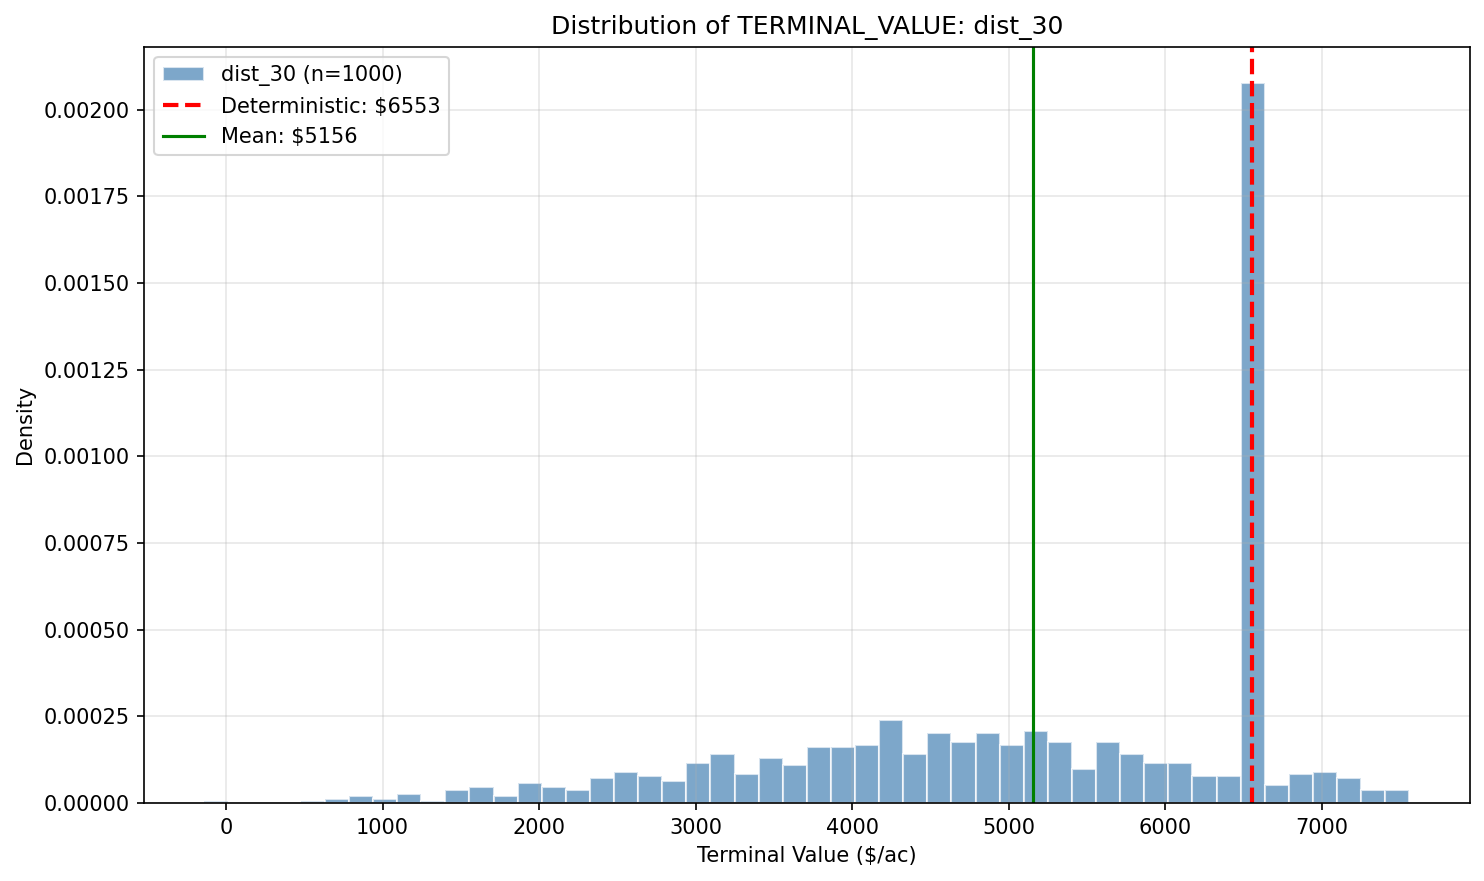
\includegraphics[width=0.7\linewidth]{../data/experiment_results/figures/histograms/dist_30_terminal_value_histogram.png}
  \caption{Terminal value distribution: \texttt{dist\_30} ($\lambda_{\text{proc}}=0$, $p_{\text{dist}}=1/30$).}
  \label{fig:hist-dist30}
\end{figure}

\begin{figure}[htbp]
  \centering
  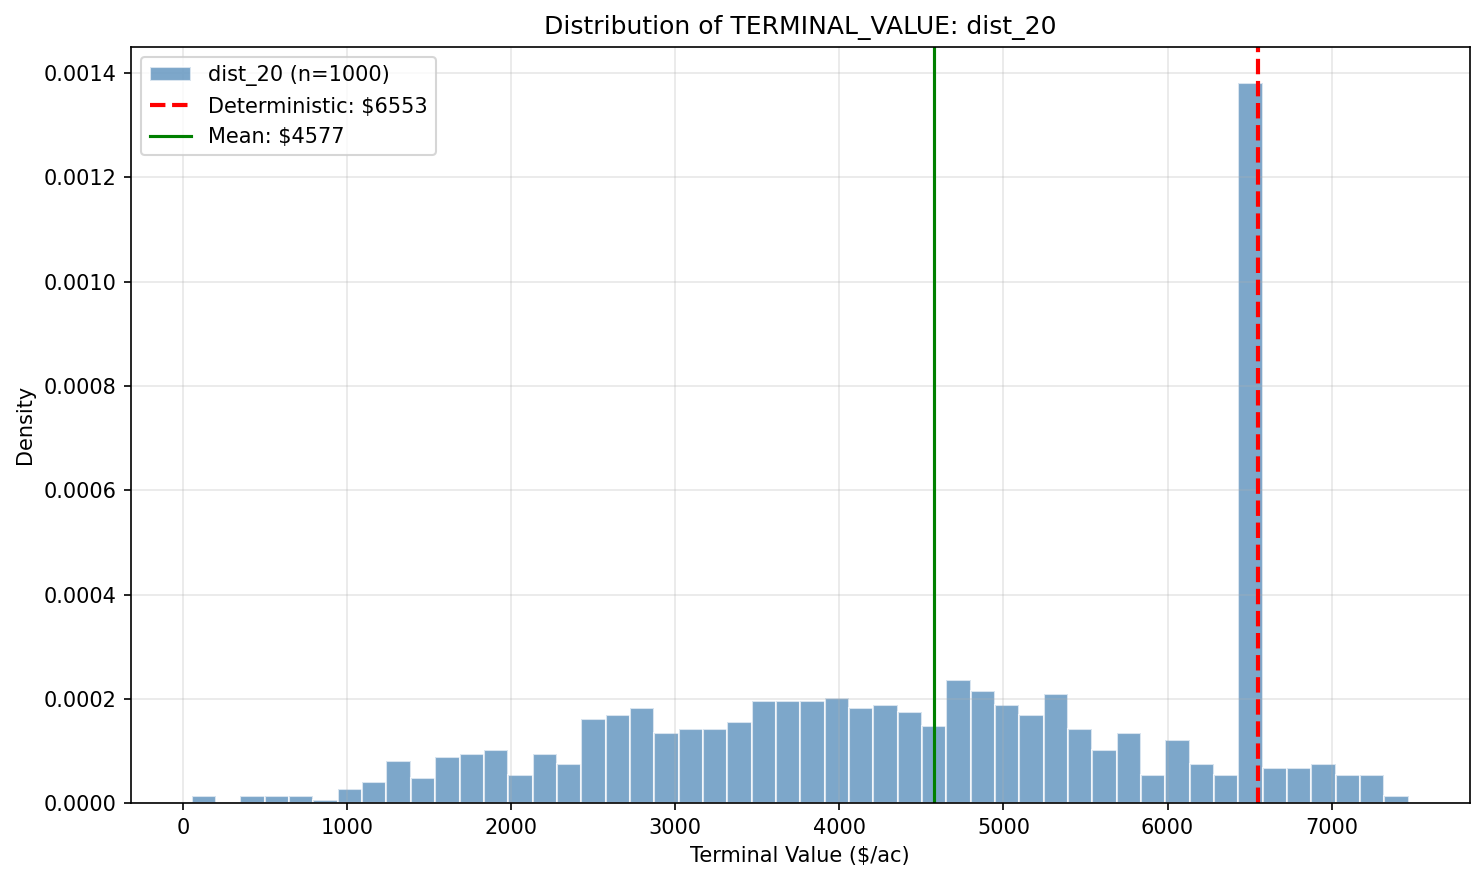
\includegraphics[width=0.7\linewidth]{../data/experiment_results/figures/histograms/dist_20_terminal_value_histogram.png}
  \caption{Terminal value distribution: \texttt{dist\_20} ($\lambda_{\text{proc}}=0$, $p_{\text{dist}}=1/20$).}
  \label{fig:hist-dist20}
\end{figure}

\begin{figure}[htbp]
  \centering
  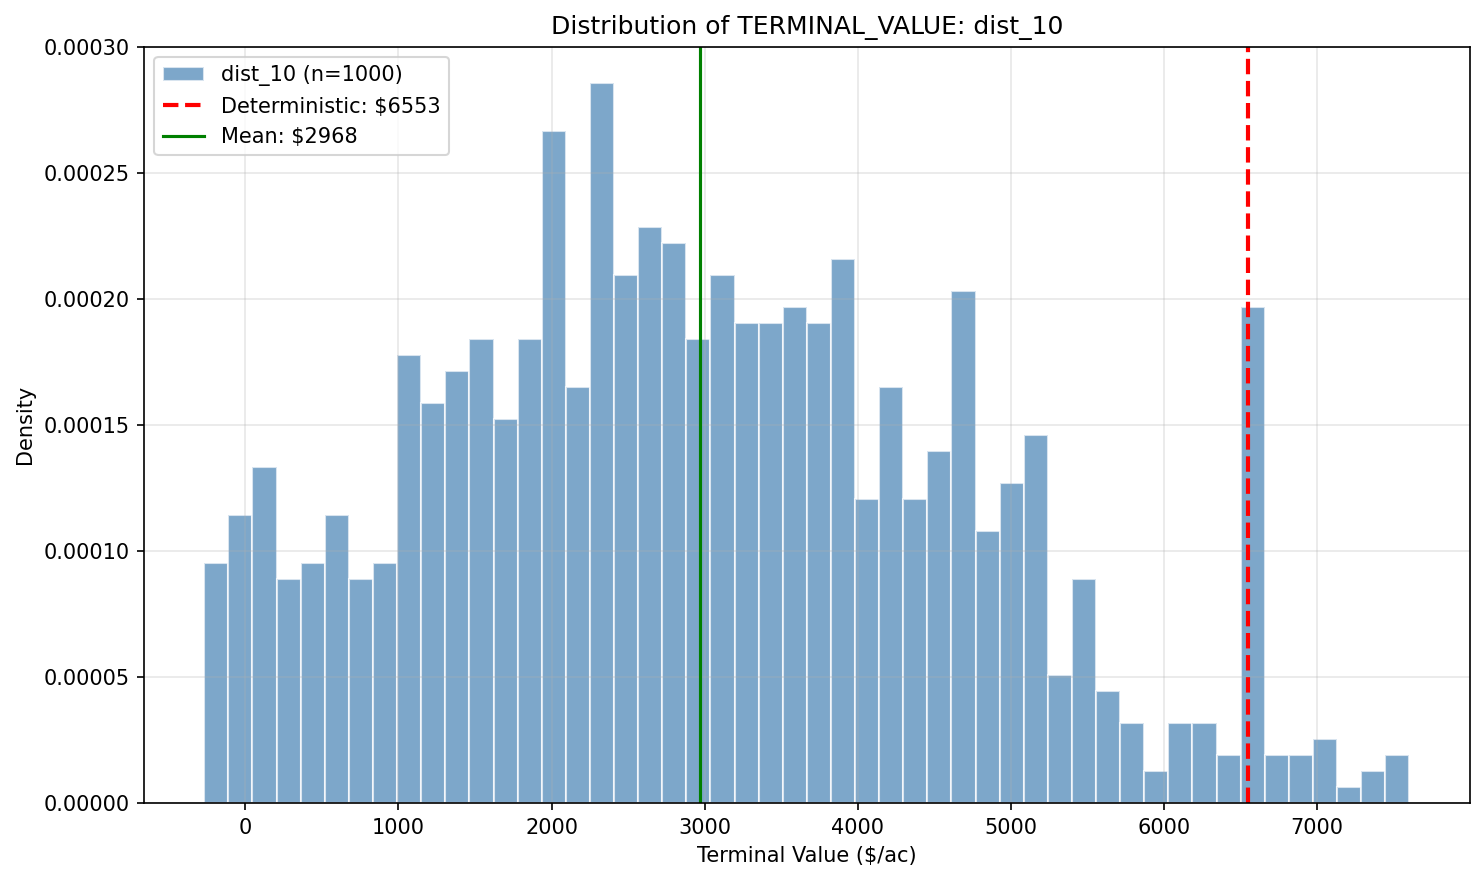
\includegraphics[width=0.7\linewidth]{../data/experiment_results/figures/histograms/dist_10_terminal_value_histogram.png}
  \caption{Terminal value distribution: \texttt{dist\_10} ($\lambda_{\text{proc}}=0$, $p_{\text{dist}}=1/10$).}
  \label{fig:hist-dist10}
\end{figure}

\clearpage
\section{Process Noise-Only Scenarios}

\begin{figure}[htbp]
  \centering
  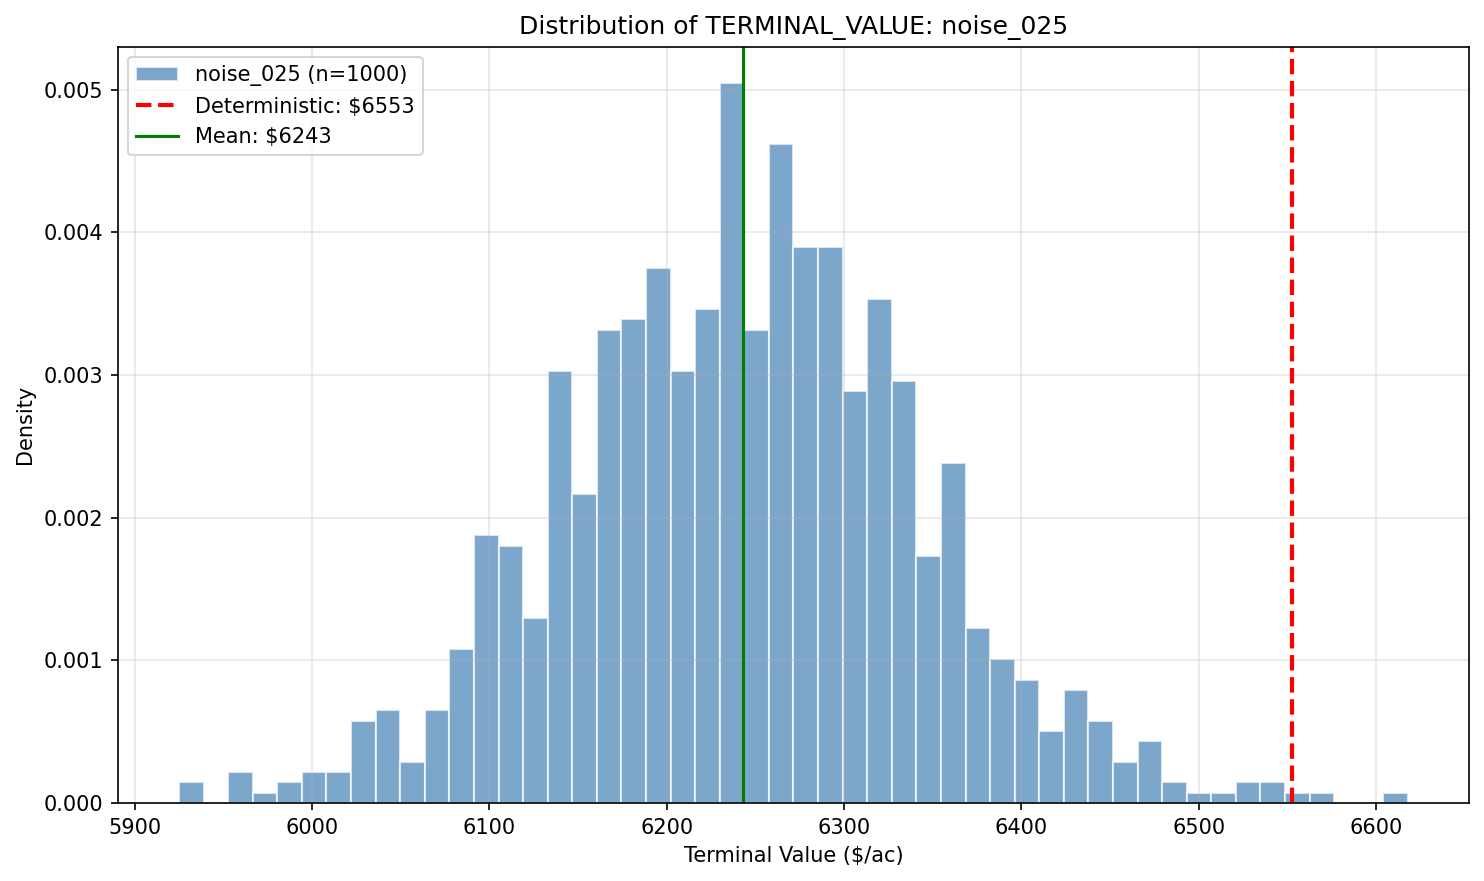
\includegraphics[width=0.7\linewidth]{../data/experiment_results/figures/histograms/noise_025_terminal_value_histogram.png}
  \caption{Terminal value distribution: \texttt{noise\_025} ($\lambda_{\text{proc}}=0.25$, $p_{\text{dist}}=0$).}
  \label{fig:hist-noise025}
\end{figure}

\begin{figure}[htbp]
  \centering
  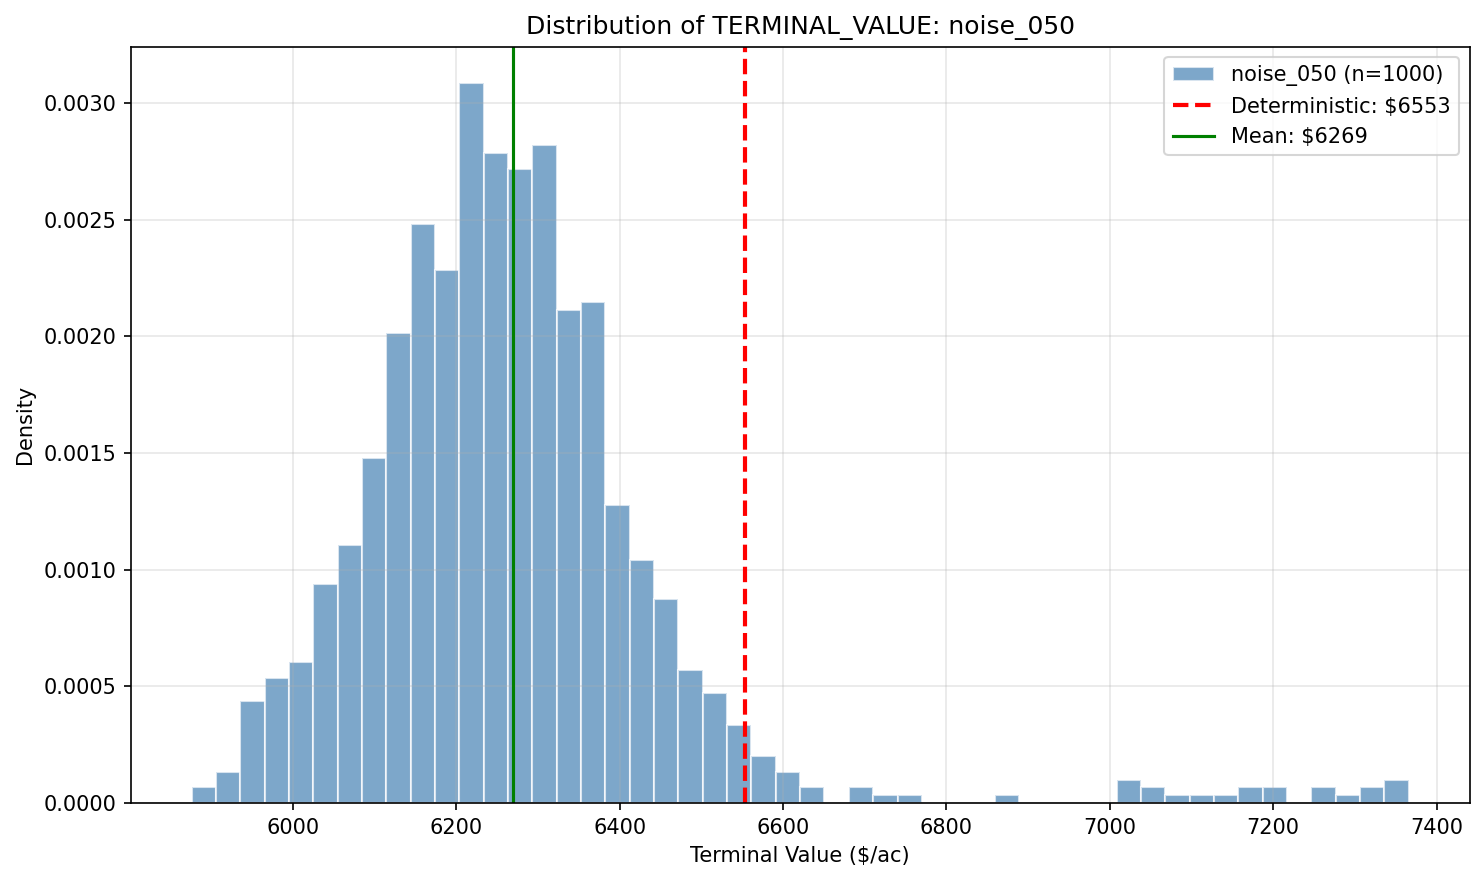
\includegraphics[width=0.7\linewidth]{../data/experiment_results/figures/histograms/noise_050_terminal_value_histogram.png}
  \caption{Terminal value distribution: \texttt{noise\_050} ($\lambda_{\text{proc}}=0.50$, $p_{\text{dist}}=0$).}
  \label{fig:hist-noise050}
\end{figure}

\begin{figure}[htbp]
  \centering
  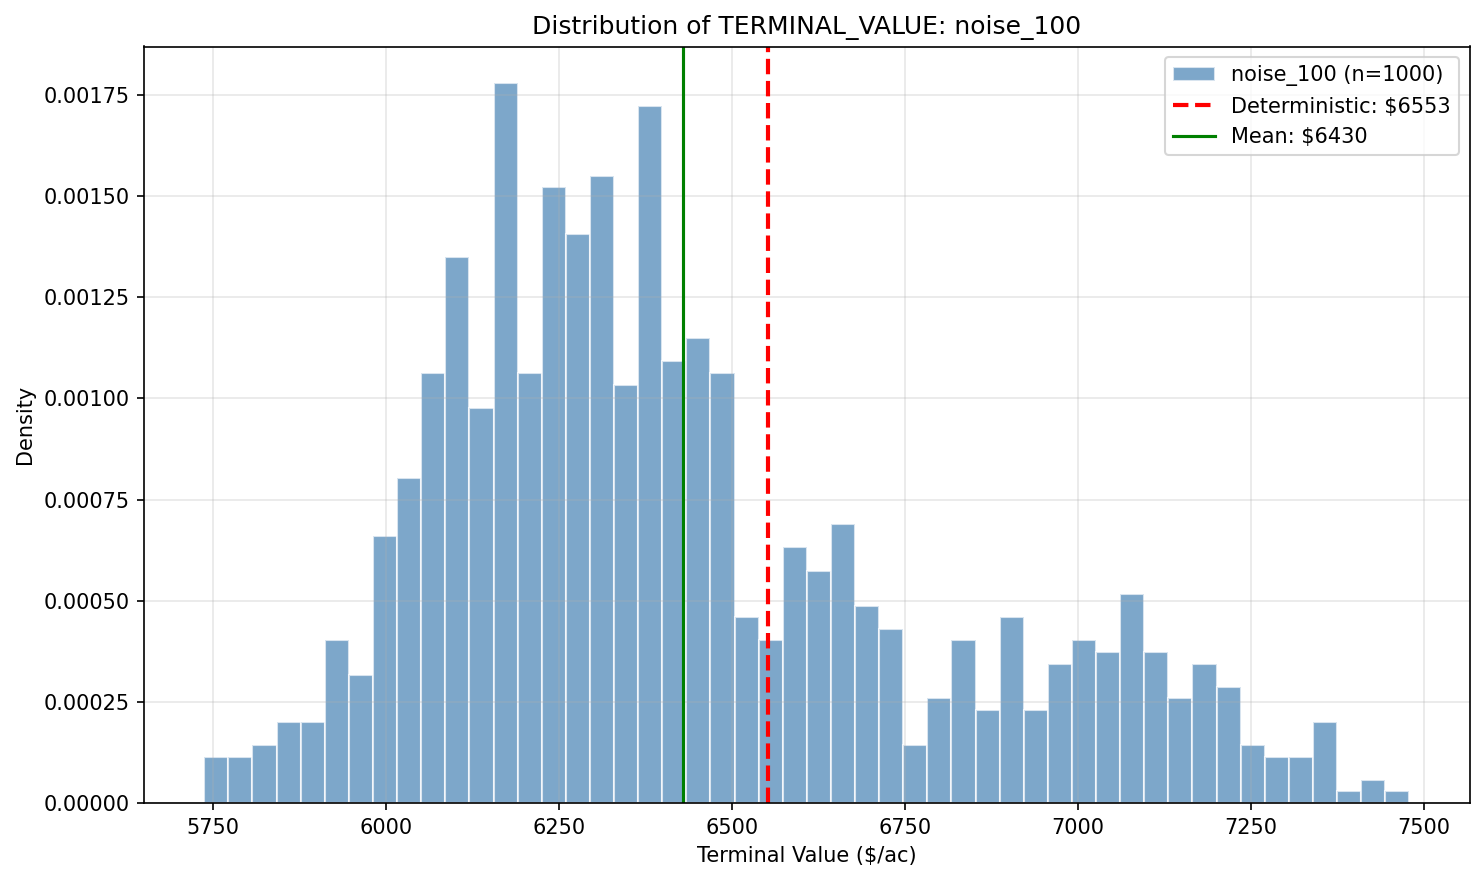
\includegraphics[width=0.7\linewidth]{../data/experiment_results/figures/histograms/noise_100_terminal_value_histogram.png}
  \caption{Terminal value distribution: \texttt{noise\_100} ($\lambda_{\text{proc}}=1.00$, $p_{\text{dist}}=0$).}
  \label{fig:hist-noise100}
\end{figure}

\clearpage
\section{Combined Scenarios: Low Noise ($\lambda_{\text{proc}}=0.25$)}

\begin{figure}[htbp]
  \centering
  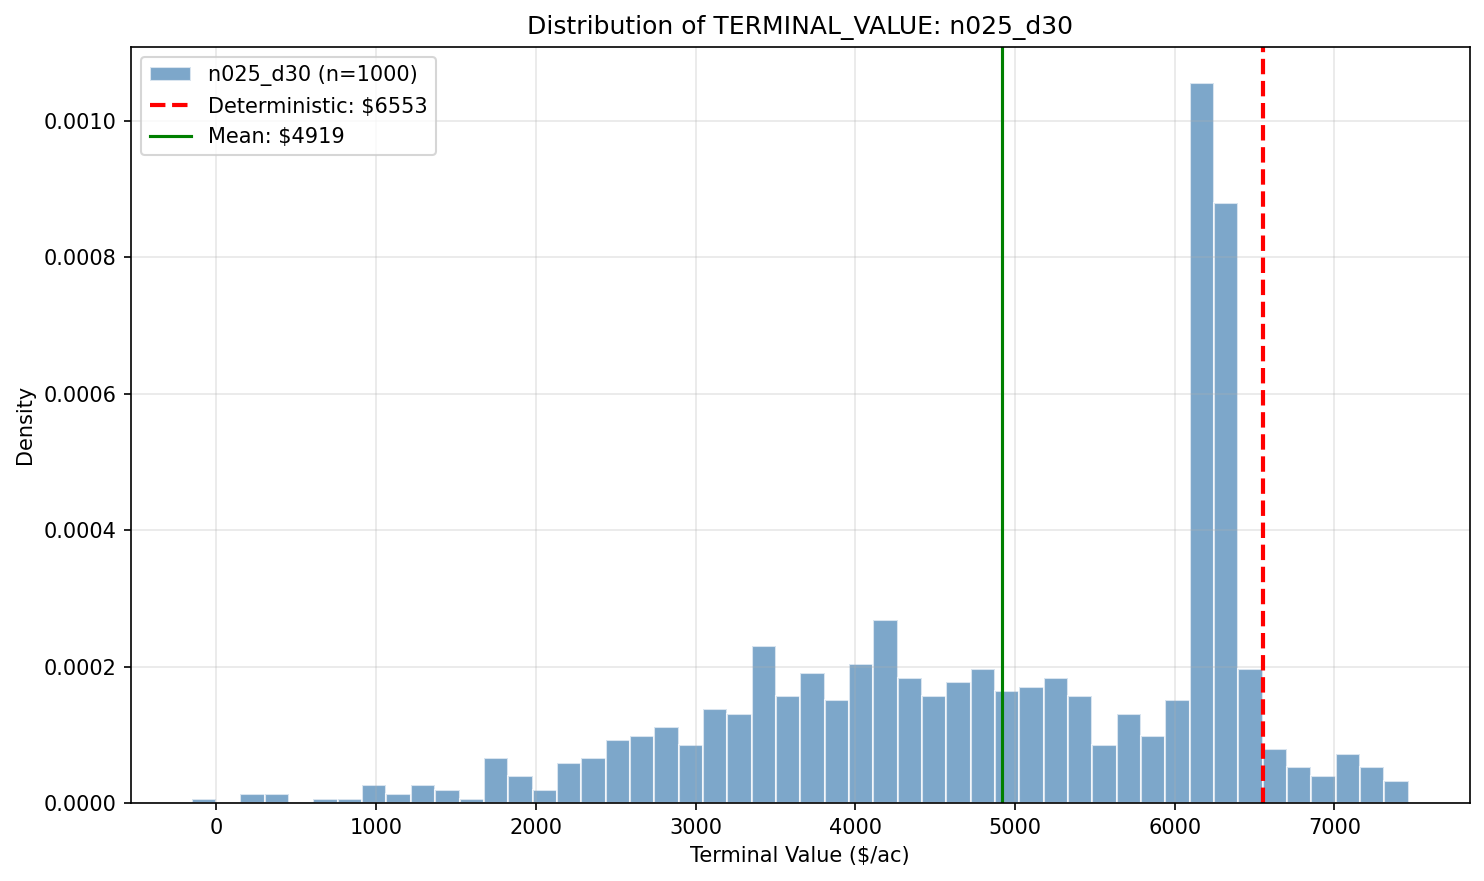
\includegraphics[width=0.7\linewidth]{../data/experiment_results/figures/histograms/n025_d30_terminal_value_histogram.png}
  \caption{Terminal value distribution: \texttt{n025\_d30} ($\lambda_{\text{proc}}=0.25$, $p_{\text{dist}}=1/30$).}
  \label{fig:hist-n025d30}
\end{figure}

\begin{figure}[htbp]
  \centering
  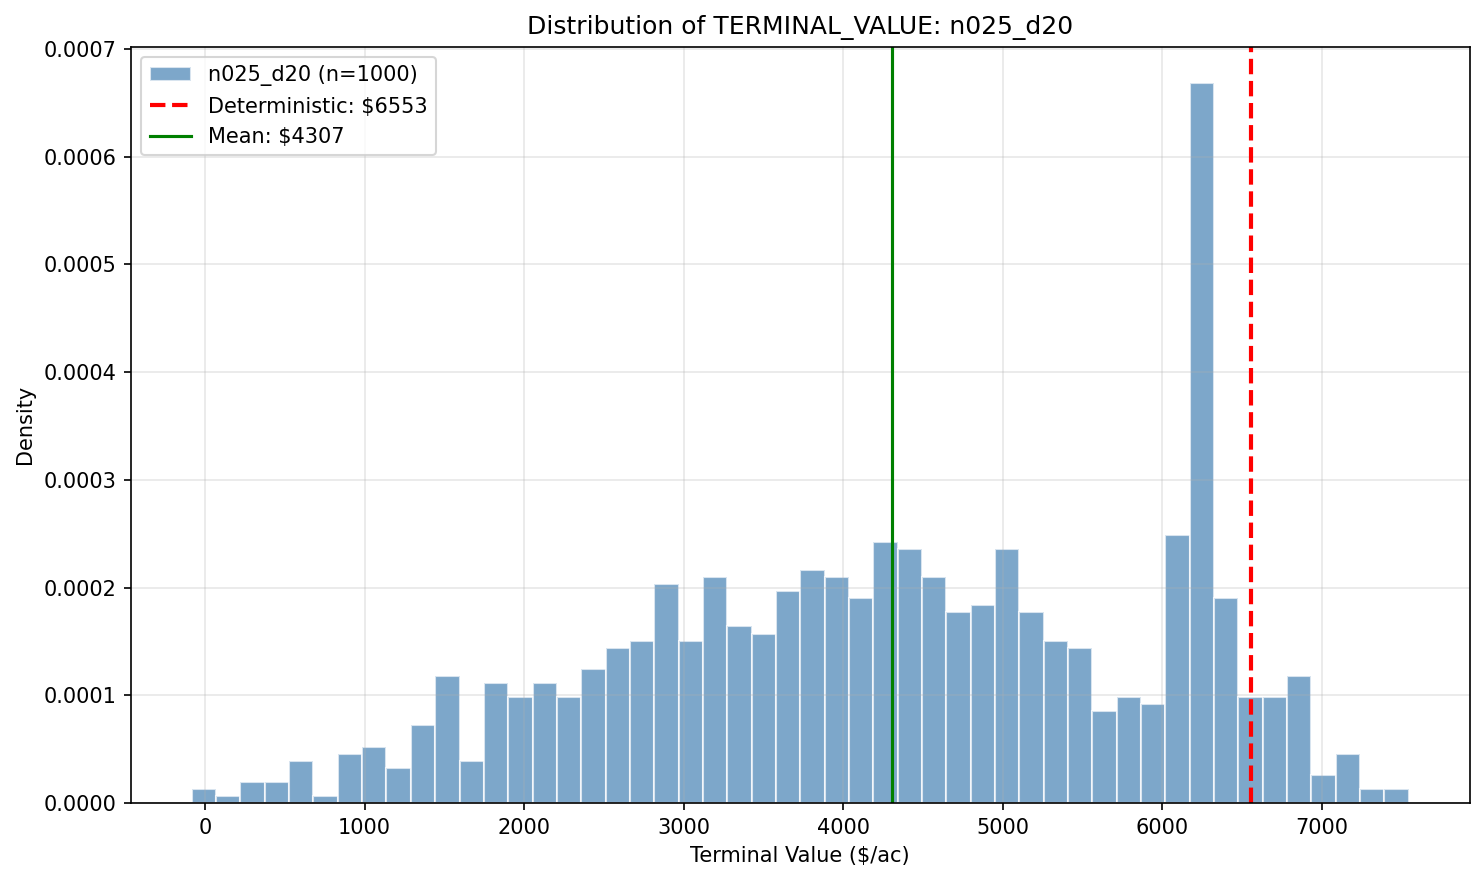
\includegraphics[width=0.7\linewidth]{../data/experiment_results/figures/histograms/n025_d20_terminal_value_histogram.png}
  \caption{Terminal value distribution: \texttt{n025\_d20} ($\lambda_{\text{proc}}=0.25$, $p_{\text{dist}}=1/20$).}
  \label{fig:hist-n025d20}
\end{figure}

\begin{figure}[htbp]
  \centering
  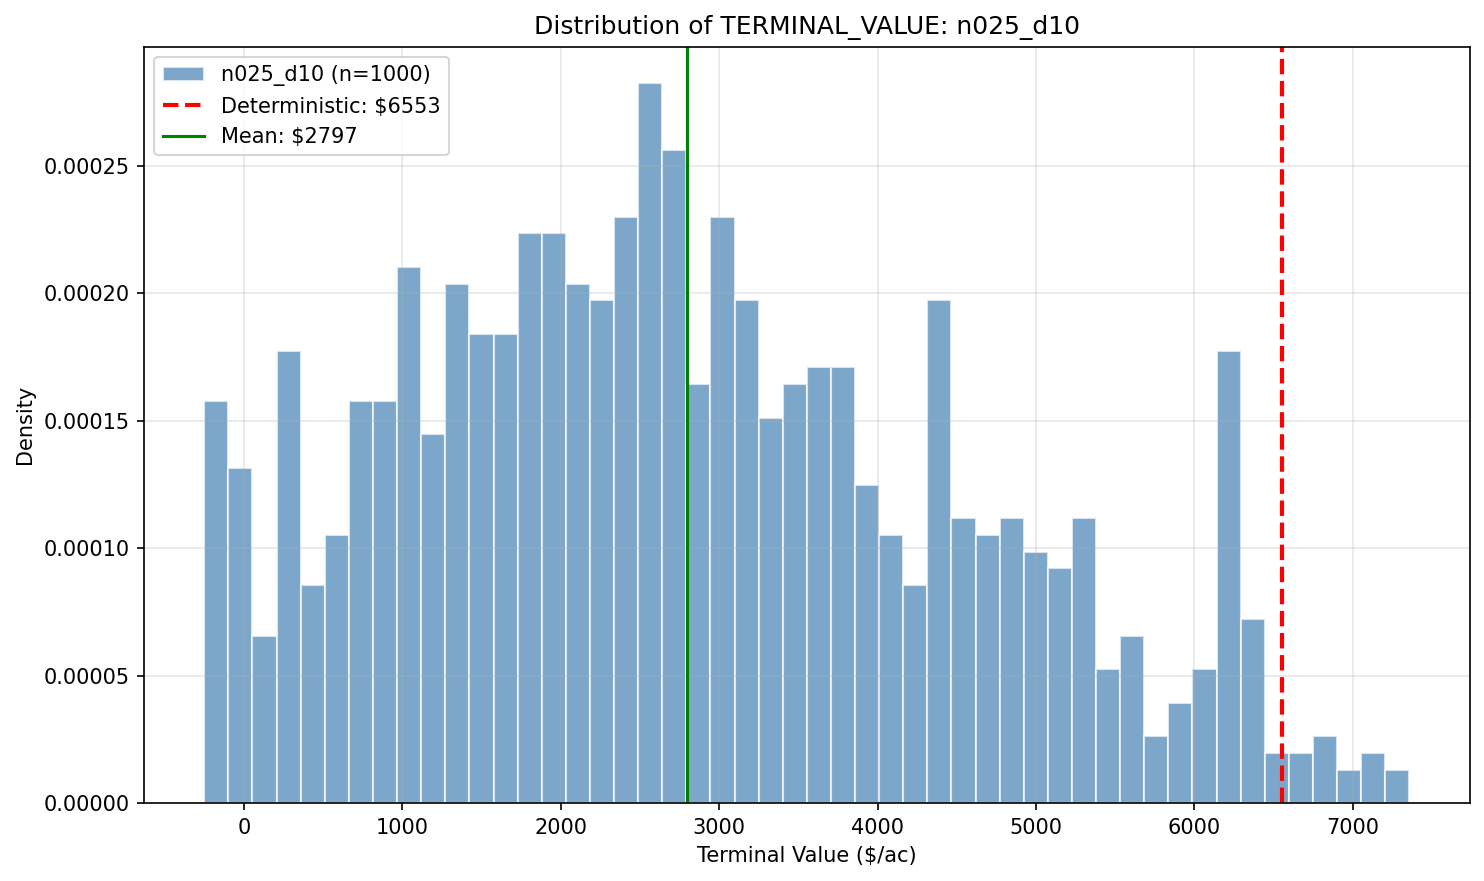
\includegraphics[width=0.7\linewidth]{../data/experiment_results/figures/histograms/n025_d10_terminal_value_histogram.png}
  \caption{Terminal value distribution: \texttt{n025\_d10} ($\lambda_{\text{proc}}=0.25$, $p_{\text{dist}}=1/10$).}
  \label{fig:hist-n025d10}
\end{figure}

\clearpage
\section{Combined Scenarios: Moderate Noise ($\lambda_{\text{proc}}=0.50$)}

\begin{figure}[htbp]
  \centering
  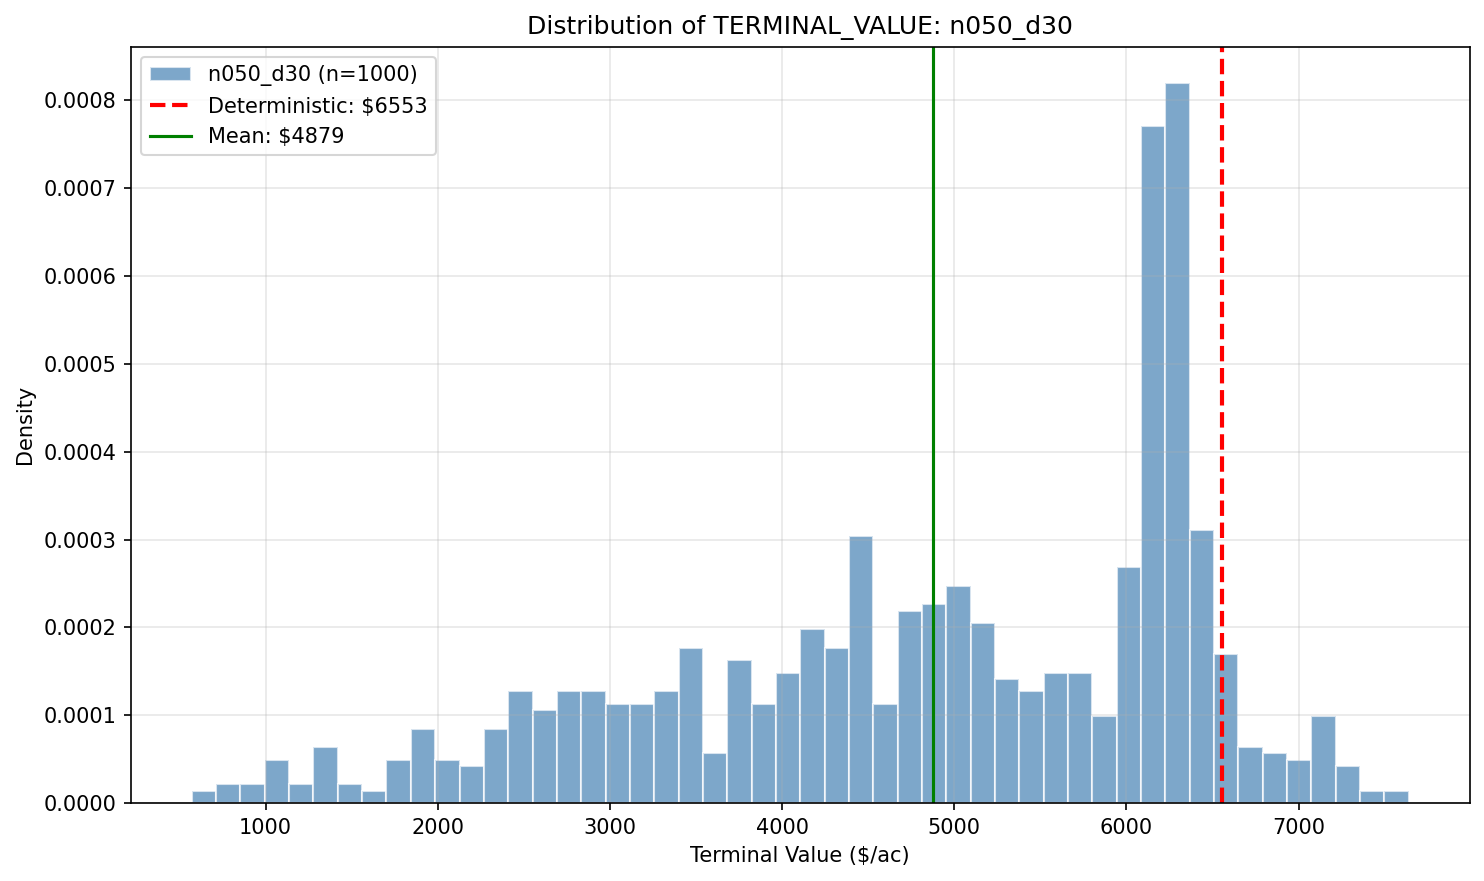
\includegraphics[width=0.7\linewidth]{../data/experiment_results/figures/histograms/n050_d30_terminal_value_histogram.png}
  \caption{Terminal value distribution: \texttt{n050\_d30} ($\lambda_{\text{proc}}=0.50$, $p_{\text{dist}}=1/30$).}
  \label{fig:hist-n050d30}
\end{figure}

\begin{figure}[htbp]
  \centering
  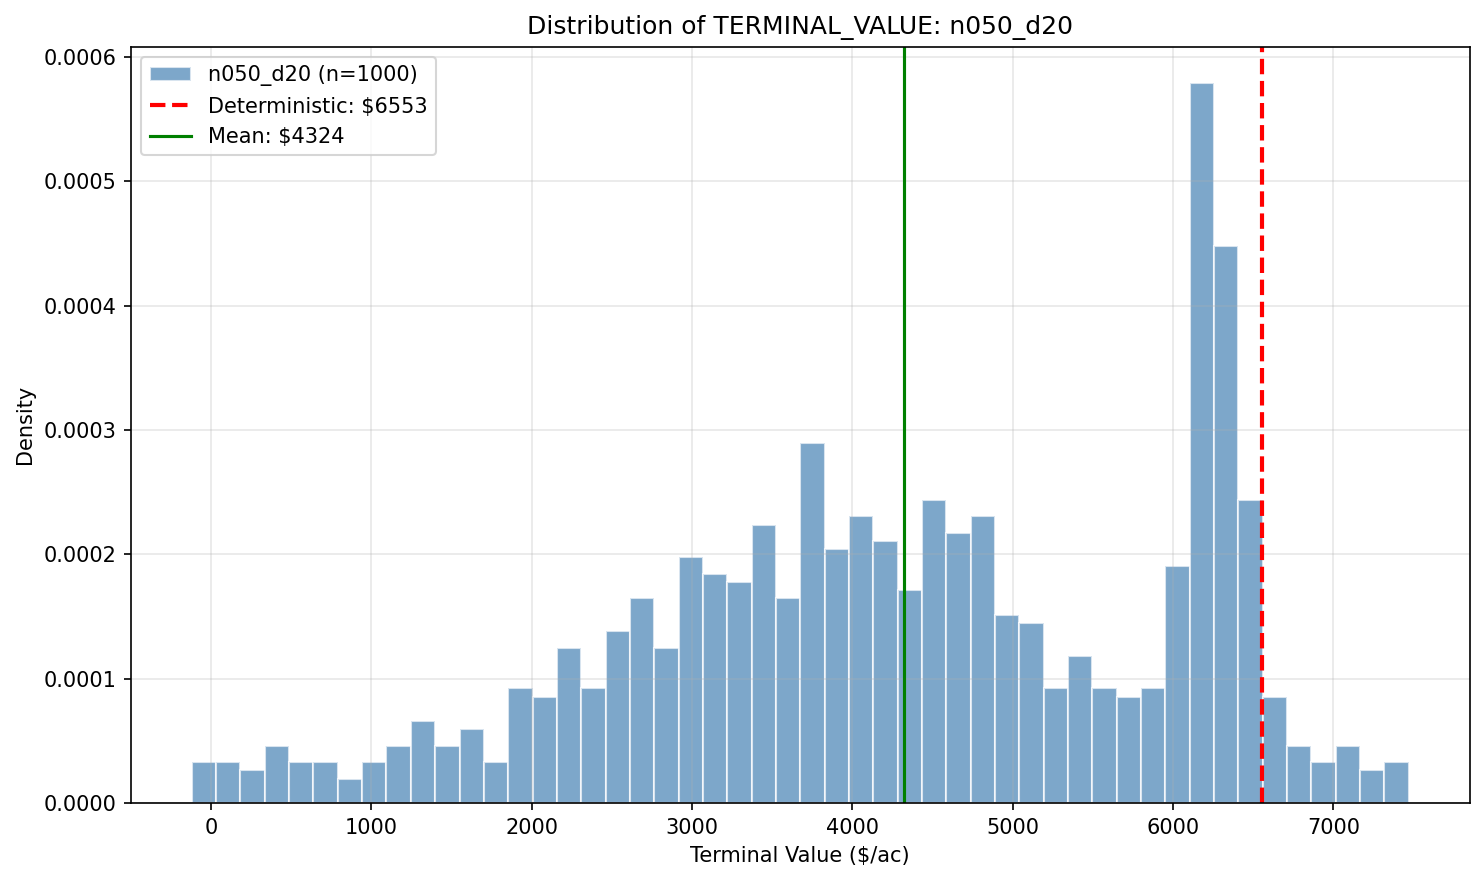
\includegraphics[width=0.7\linewidth]{../data/experiment_results/figures/histograms/n050_d20_terminal_value_histogram.png}
  \caption{Terminal value distribution: \texttt{n050\_d20} ($\lambda_{\text{proc}}=0.50$, $p_{\text{dist}}=1/20$).}
  \label{fig:hist-n050d20}
\end{figure}

\begin{figure}[htbp]
  \centering
  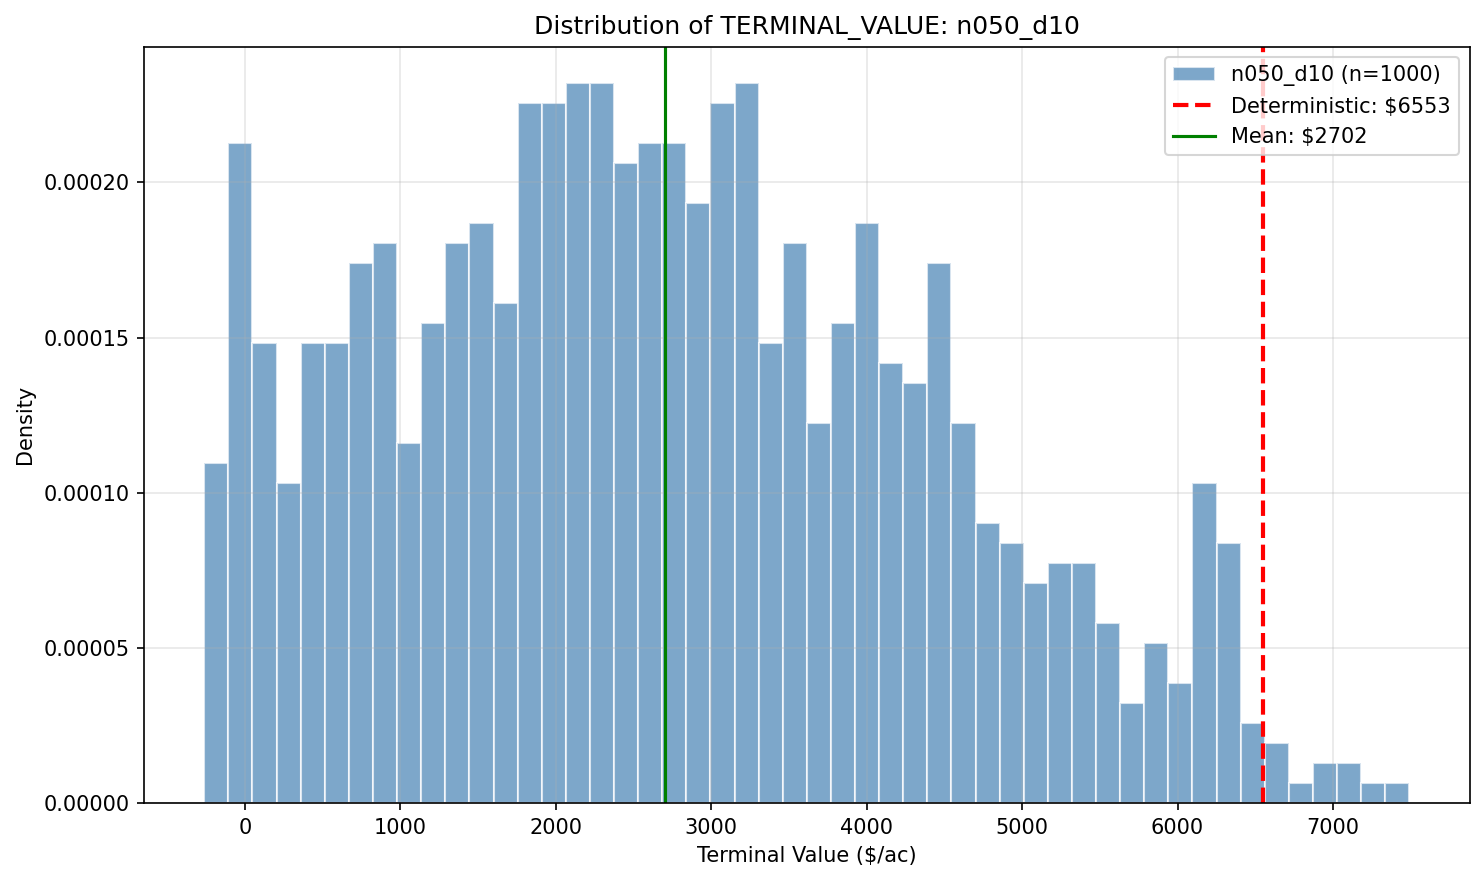
\includegraphics[width=0.7\linewidth]{../data/experiment_results/figures/histograms/n050_d10_terminal_value_histogram.png}
  \caption{Terminal value distribution: \texttt{n050\_d10} ($\lambda_{\text{proc}}=0.50$, $p_{\text{dist}}=1/10$).}
  \label{fig:hist-n050d10}
\end{figure}

\clearpage
\section{Combined Scenarios: Full Noise ($\lambda_{\text{proc}}=1.00$)}

\begin{figure}[htbp]
  \centering
  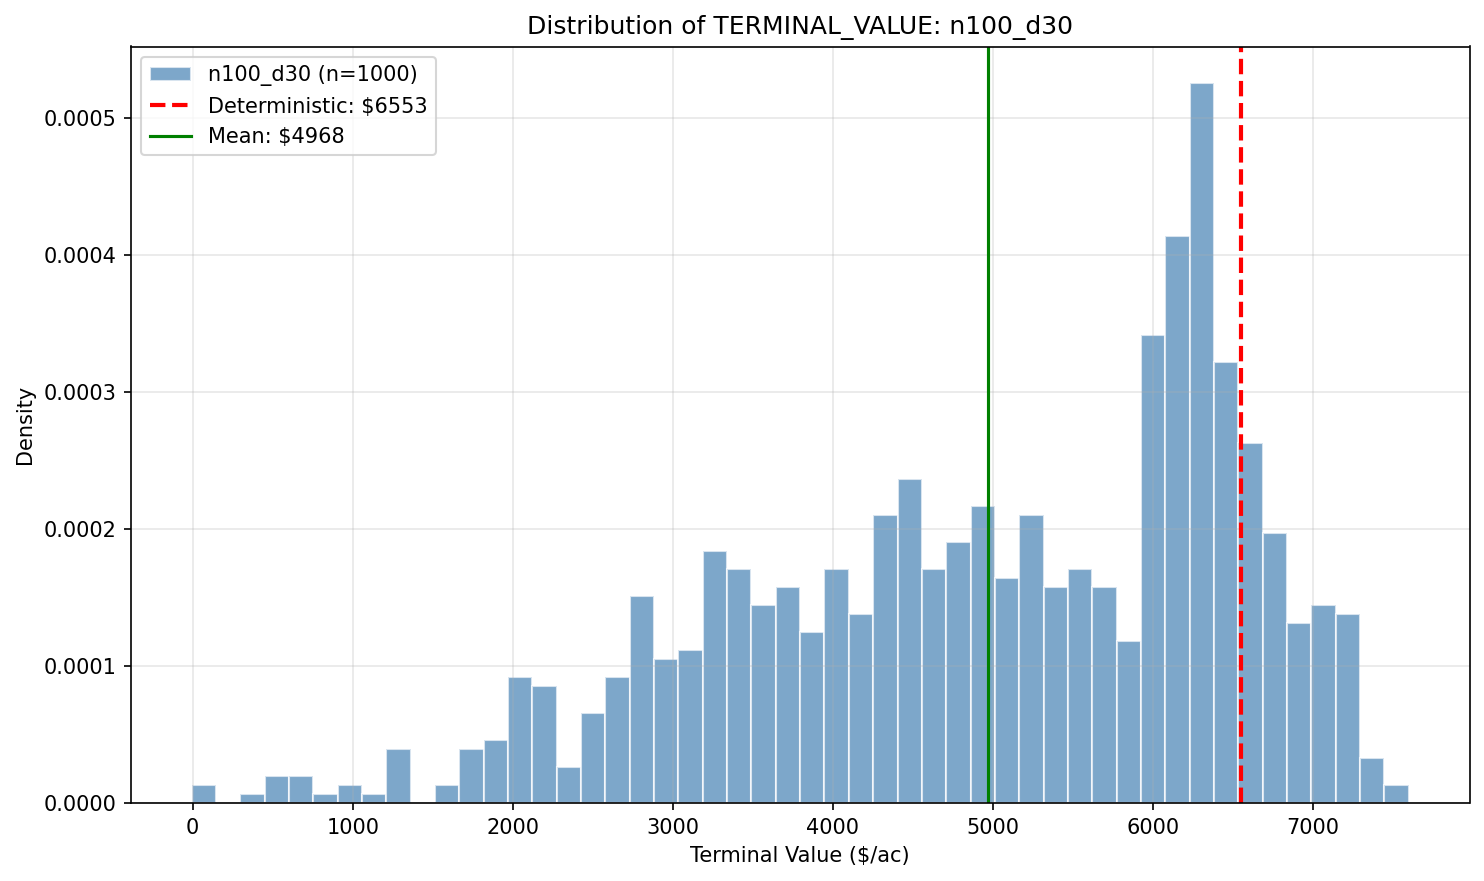
\includegraphics[width=0.7\linewidth]{../data/experiment_results/figures/histograms/n100_d30_terminal_value_histogram.png}
  \caption{Terminal value distribution: \texttt{n100\_d30} ($\lambda_{\text{proc}}=1.00$, $p_{\text{dist}}=1/30$).}
  \label{fig:hist-n100d30}
\end{figure}

\begin{figure}[htbp]
  \centering
  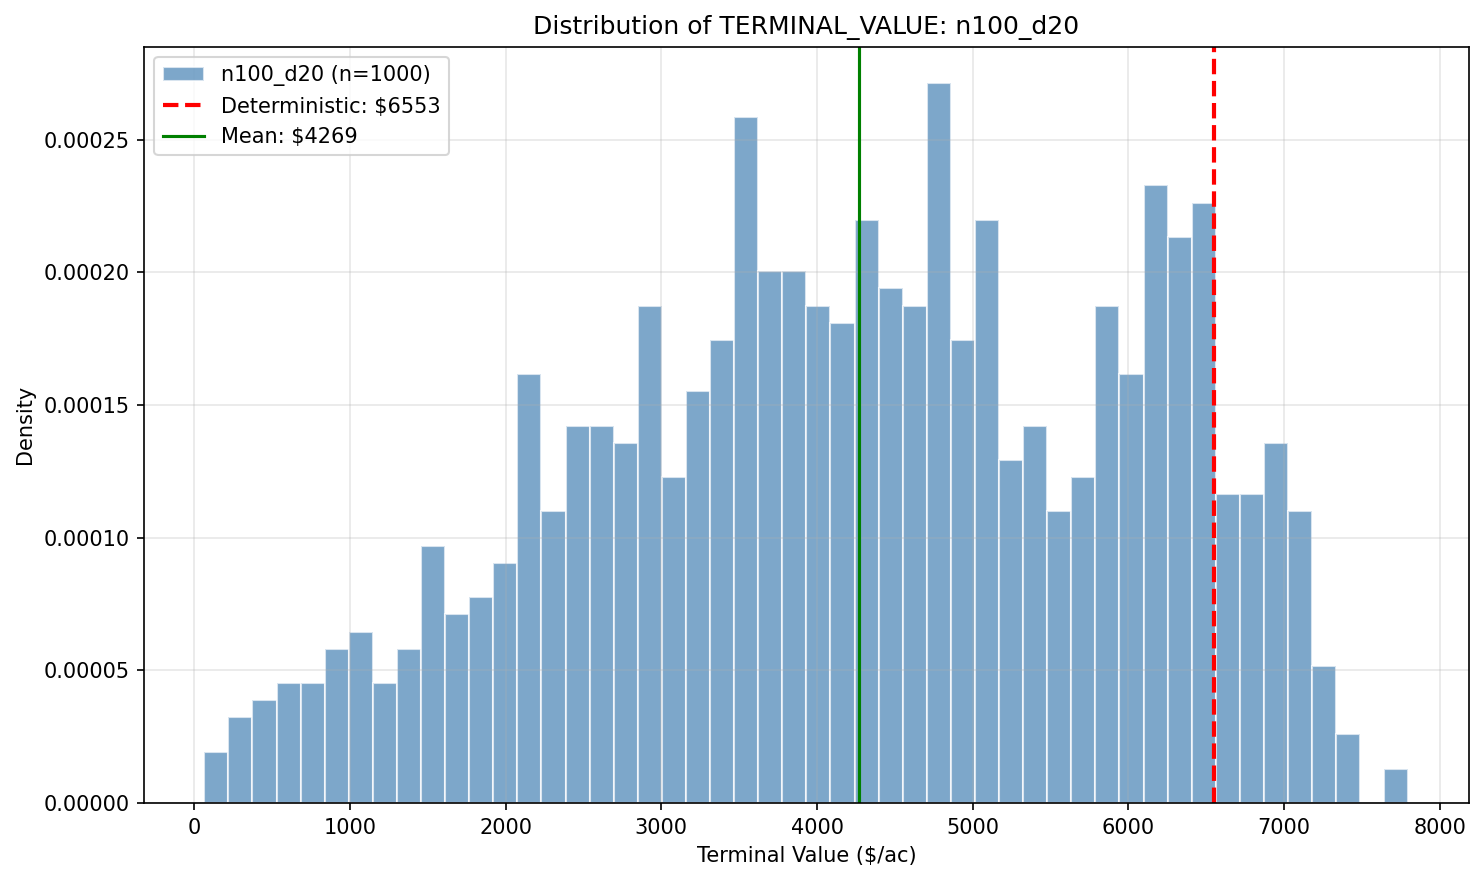
\includegraphics[width=0.7\linewidth]{../data/experiment_results/figures/histograms/n100_d20_terminal_value_histogram.png}
  \caption{Terminal value distribution: \texttt{n100\_d20} ($\lambda_{\text{proc}}=1.00$, $p_{\text{dist}}=1/20$).}
  \label{fig:hist-n100d20}
\end{figure}

\begin{figure}[htbp]
  \centering
  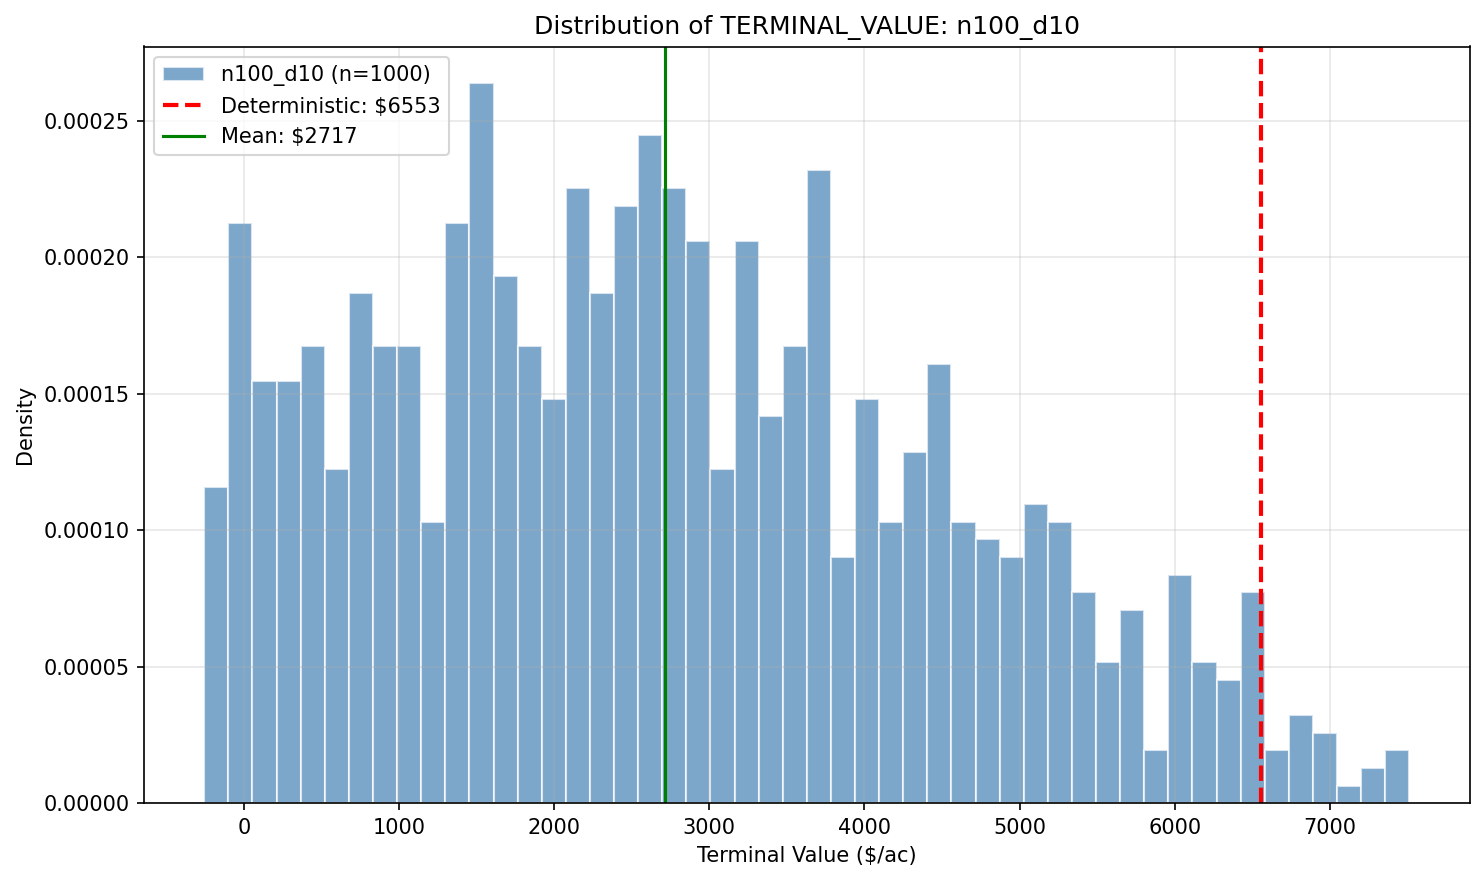
\includegraphics[width=0.7\linewidth]{../data/experiment_results/figures/histograms/n100_d10_terminal_value_histogram.png}
  \caption{Terminal value distribution: \texttt{n100\_d10} ($\lambda_{\text{proc}}=1.00$, $p_{\text{dist}}=1/10$).}
  \label{fig:hist-n100d10}
\end{figure}

\end{document}
